% Created by tikzDevice version 0.12
% !TEX encoding = UTF-8 Unicode
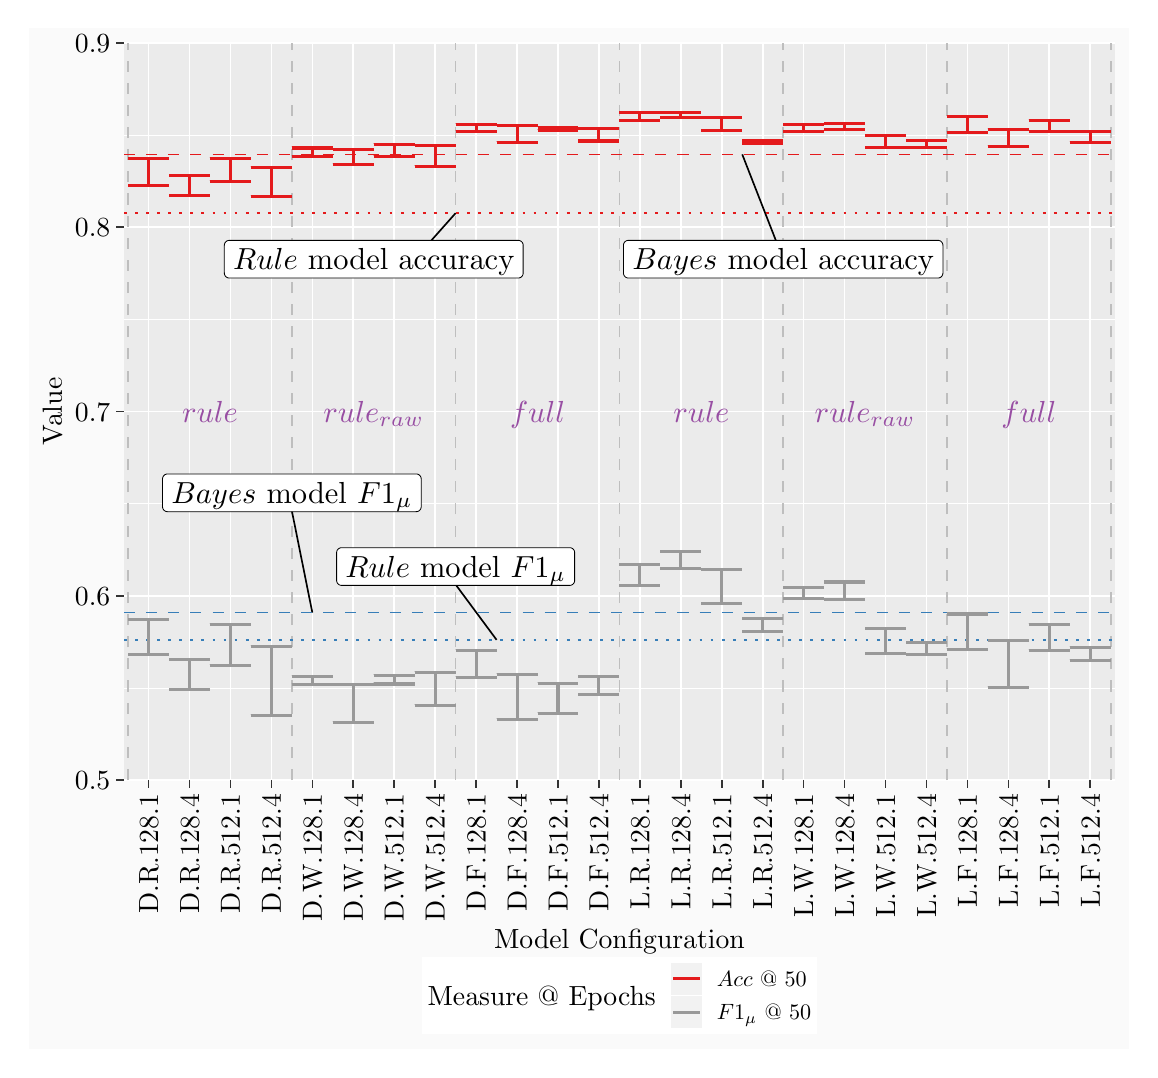
\begin{tikzpicture}[x=1pt,y=1pt]
\definecolor{fillColor}{RGB}{255,255,255}
\path[use as bounding box,fill=fillColor,fill opacity=0.00] (0,0) rectangle (398.34,369.26);
\begin{scope}
\path[clip] (  0.00,  0.00) rectangle (398.34,369.26);
\definecolor{drawColor}{RGB}{255,255,255}
\definecolor{fillColor}{gray}{0.98}

\path[draw=drawColor,line width= 0.6pt,line join=round,line cap=round,fill=fillColor] (  0.00,  0.00) rectangle (398.34,369.26);
\end{scope}
\begin{scope}
\path[clip] ( 34.81, 97.36) rectangle (392.84,363.76);
\definecolor{fillColor}{gray}{0.92}

\path[fill=fillColor] ( 34.81, 97.36) rectangle (392.84,363.76);
\definecolor{drawColor}{RGB}{255,255,255}

\path[draw=drawColor,line width= 0.3pt,line join=round] ( 34.81,130.66) --
	(392.84,130.66);

\path[draw=drawColor,line width= 0.3pt,line join=round] ( 34.81,197.26) --
	(392.84,197.26);

\path[draw=drawColor,line width= 0.3pt,line join=round] ( 34.81,263.86) --
	(392.84,263.86);

\path[draw=drawColor,line width= 0.3pt,line join=round] ( 34.81,330.46) --
	(392.84,330.46);

\path[draw=drawColor,line width= 0.6pt,line join=round] ( 34.81, 97.36) --
	(392.84, 97.36);

\path[draw=drawColor,line width= 0.6pt,line join=round] ( 34.81,163.96) --
	(392.84,163.96);

\path[draw=drawColor,line width= 0.6pt,line join=round] ( 34.81,230.56) --
	(392.84,230.56);

\path[draw=drawColor,line width= 0.6pt,line join=round] ( 34.81,297.16) --
	(392.84,297.16);

\path[draw=drawColor,line width= 0.6pt,line join=round] ( 34.81,363.76) --
	(392.84,363.76);

\path[draw=drawColor,line width= 0.6pt,line join=round] ( 43.68, 97.36) --
	( 43.68,363.76);

\path[draw=drawColor,line width= 0.6pt,line join=round] ( 58.48, 97.36) --
	( 58.48,363.76);

\path[draw=drawColor,line width= 0.6pt,line join=round] ( 73.27, 97.36) --
	( 73.27,363.76);

\path[draw=drawColor,line width= 0.6pt,line join=round] ( 88.07, 97.36) --
	( 88.07,363.76);

\path[draw=drawColor,line width= 0.6pt,line join=round] (102.86, 97.36) --
	(102.86,363.76);

\path[draw=drawColor,line width= 0.6pt,line join=round] (117.66, 97.36) --
	(117.66,363.76);

\path[draw=drawColor,line width= 0.6pt,line join=round] (132.45, 97.36) --
	(132.45,363.76);

\path[draw=drawColor,line width= 0.6pt,line join=round] (147.25, 97.36) --
	(147.25,363.76);

\path[draw=drawColor,line width= 0.6pt,line join=round] (162.04, 97.36) --
	(162.04,363.76);

\path[draw=drawColor,line width= 0.6pt,line join=round] (176.84, 97.36) --
	(176.84,363.76);

\path[draw=drawColor,line width= 0.6pt,line join=round] (191.63, 97.36) --
	(191.63,363.76);

\path[draw=drawColor,line width= 0.6pt,line join=round] (206.42, 97.36) --
	(206.42,363.76);

\path[draw=drawColor,line width= 0.6pt,line join=round] (221.22, 97.36) --
	(221.22,363.76);

\path[draw=drawColor,line width= 0.6pt,line join=round] (236.01, 97.36) --
	(236.01,363.76);

\path[draw=drawColor,line width= 0.6pt,line join=round] (250.81, 97.36) --
	(250.81,363.76);

\path[draw=drawColor,line width= 0.6pt,line join=round] (265.60, 97.36) --
	(265.60,363.76);

\path[draw=drawColor,line width= 0.6pt,line join=round] (280.40, 97.36) --
	(280.40,363.76);

\path[draw=drawColor,line width= 0.6pt,line join=round] (295.19, 97.36) --
	(295.19,363.76);

\path[draw=drawColor,line width= 0.6pt,line join=round] (309.99, 97.36) --
	(309.99,363.76);

\path[draw=drawColor,line width= 0.6pt,line join=round] (324.78, 97.36) --
	(324.78,363.76);

\path[draw=drawColor,line width= 0.6pt,line join=round] (339.58, 97.36) --
	(339.58,363.76);

\path[draw=drawColor,line width= 0.6pt,line join=round] (354.37, 97.36) --
	(354.37,363.76);

\path[draw=drawColor,line width= 0.6pt,line join=round] (369.17, 97.36) --
	(369.17,363.76);

\path[draw=drawColor,line width= 0.6pt,line join=round] (383.96, 97.36) --
	(383.96,363.76);
\definecolor{drawColor}{RGB}{190,190,190}

\path[draw=drawColor,line width= 0.6pt,dash pattern=on 4pt off 4pt ,line join=round] ( 36.29, 97.36) -- ( 36.29,363.76);

\path[draw=drawColor,line width= 0.6pt,dash pattern=on 4pt off 4pt ,line join=round] ( 95.46, 97.36) -- ( 95.46,363.76);

\path[draw=drawColor,line width= 0.6pt,dash pattern=on 4pt off 4pt ,line join=round] (154.64, 97.36) -- (154.64,363.76);

\path[draw=drawColor,line width= 0.6pt,dash pattern=on 4pt off 4pt ,line join=round] (213.82, 97.36) -- (213.82,363.76);

\path[draw=drawColor,line width= 0.6pt,dash pattern=on 4pt off 4pt ,line join=round] (273.00, 97.36) -- (273.00,363.76);

\path[draw=drawColor,line width= 0.6pt,dash pattern=on 4pt off 4pt ,line join=round] (332.18, 97.36) -- (332.18,363.76);

\path[draw=drawColor,line width= 0.6pt,dash pattern=on 4pt off 4pt ,line join=round] (391.36, 97.36) -- (391.36,363.76);
\definecolor{drawColor}{RGB}{152,78,163}

\node[text=drawColor,anchor=base,inner sep=0pt, outer sep=0pt, scale=  1.10] at ( 65.87,226.76) {\(rule\)};

\node[text=drawColor,anchor=base,inner sep=0pt, outer sep=0pt, scale=  1.10] at (125.05,226.76) {\(rule_{raw}\)};

\node[text=drawColor,anchor=base,inner sep=0pt, outer sep=0pt, scale=  1.10] at (184.23,226.76) {\(full\)};

\node[text=drawColor,anchor=base,inner sep=0pt, outer sep=0pt, scale=  1.10] at (243.41,226.76) {\(rule\)};

\node[text=drawColor,anchor=base,inner sep=0pt, outer sep=0pt, scale=  1.10] at (302.59,226.76) {\(rule_{raw}\)};

\node[text=drawColor,anchor=base,inner sep=0pt, outer sep=0pt, scale=  1.10] at (361.77,226.76) {\(full\)};
\definecolor{drawColor}{RGB}{0,0,0}

\path[draw=drawColor,line width= 0.6pt,line join=round] (139.85,285.60) --
	(154.64,302.25);

\path[draw=drawColor,line width= 0.6pt,line join=round] (258.21,323.47) --
	(273.00,285.60);

\path[draw=drawColor,line width= 0.6pt,line join=round] (154.64,168.03) --
	(169.44,148.05);

\path[draw=drawColor,line width= 0.6pt,line join=round] ( 95.46,194.67) --
	(102.86,157.89);
\definecolor{fillColor}{RGB}{255,255,255}

\path[draw=drawColor,line width= 0.3pt,line join=round,line cap=round,fill=fillColor] ( 50.54,194.36) --
	(140.39,194.36) --
	(140.32,194.37) --
	(140.61,194.38) --
	(140.89,194.44) --
	(141.17,194.54) --
	(141.42,194.68) --
	(141.64,194.87) --
	(141.84,195.09) --
	(141.99,195.33) --
	(142.11,195.60) --
	(142.17,195.88) --
	(142.20,196.17) --
	(142.20,196.17) --
	(142.20,206.18) --
	(142.20,206.18) --
	(142.17,206.47) --
	(142.11,206.76) --
	(141.99,207.02) --
	(141.84,207.27) --
	(141.64,207.49) --
	(141.42,207.67) --
	(141.17,207.82) --
	(140.89,207.92) --
	(140.61,207.98) --
	(140.39,207.99) --
	( 50.54,207.99) --
	( 50.75,207.98) --
	( 50.46,207.99) --
	( 50.18,207.95) --
	( 49.90,207.87) --
	( 49.63,207.75) --
	( 49.39,207.58) --
	( 49.18,207.38) --
	( 49.01,207.15) --
	( 48.88,206.89) --
	( 48.78,206.62) --
	( 48.74,206.33) --
	( 48.73,206.18) --
	( 48.73,196.17) --
	( 48.74,196.32) --
	( 48.74,196.03) --
	( 48.78,195.74) --
	( 48.88,195.46) --
	( 49.01,195.21) --
	( 49.18,194.97) --
	( 49.39,194.77) --
	( 49.63,194.61) --
	( 49.90,194.48) --
	( 50.18,194.40) --
	( 50.46,194.37) --
	cycle;
\end{scope}
\begin{scope}
\path[clip] ( 34.81, 97.36) rectangle (392.84,363.76);
\definecolor{drawColor}{RGB}{0,0,0}

\node[text=drawColor,anchor=base,inner sep=0pt, outer sep=0pt, scale=  1.10] at ( 95.46,197.38) {\(Bayes\) model \(F1_\mu\)};
\definecolor{fillColor}{RGB}{255,255,255}

\path[draw=drawColor,line width= 0.3pt,line join=round,line cap=round,fill=fillColor] (113.44,167.72) --
	(195.85,167.72) --
	(195.77,167.73) --
	(196.06,167.74) --
	(196.35,167.80) --
	(196.62,167.90) --
	(196.87,168.04) --
	(197.10,168.23) --
	(197.29,168.45) --
	(197.45,168.69) --
	(197.56,168.96) --
	(197.63,169.24) --
	(197.65,169.53) --
	(197.65,169.53) --
	(197.65,179.54) --
	(197.65,179.54) --
	(197.63,179.83) --
	(197.56,180.12) --
	(197.45,180.38) --
	(197.29,180.63) --
	(197.10,180.85) --
	(196.87,181.03) --
	(196.62,181.18) --
	(196.35,181.28) --
	(196.06,181.34) --
	(195.85,181.35) --
	(113.44,181.35) --
	(113.66,181.34) --
	(113.37,181.35) --
	(113.08,181.31) --
	(112.80,181.23) --
	(112.54,181.11) --
	(112.30,180.94) --
	(112.09,180.74) --
	(111.91,180.51) --
	(111.78,180.25) --
	(111.69,179.98) --
	(111.64,179.69) --
	(111.63,179.54) --
	(111.63,169.53) --
	(111.64,169.68) --
	(111.64,169.39) --
	(111.69,169.10) --
	(111.78,168.82) --
	(111.91,168.57) --
	(112.09,168.33) --
	(112.30,168.13) --
	(112.54,167.97) --
	(112.80,167.84) --
	(113.08,167.76) --
	(113.37,167.73) --
	cycle;
\end{scope}
\begin{scope}
\path[clip] ( 34.81, 97.36) rectangle (392.84,363.76);
\definecolor{drawColor}{RGB}{0,0,0}

\node[text=drawColor,anchor=base,inner sep=0pt, outer sep=0pt, scale=  1.10] at (154.64,170.74) {\(Rule\) model \(F1_\mu\)};
\definecolor{fillColor}{RGB}{255,255,255}

\path[draw=drawColor,line width= 0.3pt,line join=round,line cap=round,fill=fillColor] ( 72.87,278.78) --
	(177.24,278.78) --
	(177.16,278.79) --
	(177.46,278.80) --
	(177.74,278.86) --
	(178.01,278.96) --
	(178.26,279.10) --
	(178.49,279.29) --
	(178.68,279.51) --
	(178.84,279.75) --
	(178.95,280.02) --
	(179.02,280.30) --
	(179.04,280.59) --
	(179.04,280.59) --
	(179.04,290.60) --
	(179.04,290.60) --
	(179.02,290.89) --
	(178.95,291.18) --
	(178.84,291.44) --
	(178.68,291.69) --
	(178.49,291.91) --
	(178.26,292.09) --
	(178.01,292.24) --
	(177.74,292.34) --
	(177.46,292.40) --
	(177.24,292.41) --
	( 72.87,292.41) --
	( 73.09,292.40) --
	( 72.80,292.41) --
	( 72.51,292.37) --
	( 72.23,292.29) --
	( 71.97,292.17) --
	( 71.73,292.00) --
	( 71.52,291.80) --
	( 71.34,291.57) --
	( 71.21,291.31) --
	( 71.12,291.04) --
	( 71.07,290.75) --
	( 71.06,290.60) --
	( 71.06,280.59) --
	( 71.07,280.74) --
	( 71.07,280.45) --
	( 71.12,280.16) --
	( 71.21,279.88) --
	( 71.34,279.63) --
	( 71.52,279.39) --
	( 71.73,279.19) --
	( 71.97,279.03) --
	( 72.23,278.90) --
	( 72.51,278.82) --
	( 72.80,278.79) --
	cycle;
\end{scope}
\begin{scope}
\path[clip] ( 34.81, 97.36) rectangle (392.84,363.76);
\definecolor{drawColor}{RGB}{0,0,0}

\node[text=drawColor,anchor=base,inner sep=0pt, outer sep=0pt, scale=  1.10] at (125.05,281.80) {\(Rule\) model accuracy};
\definecolor{fillColor}{RGB}{255,255,255}

\path[draw=drawColor,line width= 0.3pt,line join=round,line cap=round,fill=fillColor] (217.09,278.78) --
	(328.91,278.78) --
	(328.84,278.79) --
	(329.13,278.80) --
	(329.41,278.86) --
	(329.68,278.96) --
	(329.94,279.10) --
	(330.16,279.29) --
	(330.35,279.51) --
	(330.51,279.75) --
	(330.62,280.02) --
	(330.69,280.30) --
	(330.72,280.59) --
	(330.72,280.59) --
	(330.72,290.60) --
	(330.72,290.60) --
	(330.69,290.89) --
	(330.62,291.18) --
	(330.51,291.44) --
	(330.35,291.69) --
	(330.16,291.91) --
	(329.94,292.09) --
	(329.68,292.24) --
	(329.41,292.34) --
	(329.13,292.40) --
	(328.91,292.41) --
	(217.09,292.41) --
	(217.31,292.40) --
	(217.02,292.41) --
	(216.73,292.37) --
	(216.45,292.29) --
	(216.19,292.17) --
	(215.95,292.00) --
	(215.74,291.80) --
	(215.57,291.57) --
	(215.43,291.31) --
	(215.34,291.04) --
	(215.29,290.75) --
	(215.29,290.60) --
	(215.29,280.59) --
	(215.29,280.74) --
	(215.29,280.45) --
	(215.34,280.16) --
	(215.43,279.88) --
	(215.57,279.63) --
	(215.74,279.39) --
	(215.95,279.19) --
	(216.19,279.03) --
	(216.45,278.90) --
	(216.73,278.82) --
	(217.02,278.79) --
	cycle;
\end{scope}
\begin{scope}
\path[clip] ( 34.81, 97.36) rectangle (392.84,363.76);
\definecolor{drawColor}{RGB}{0,0,0}

\node[text=drawColor,anchor=base,inner sep=0pt, outer sep=0pt, scale=  1.10] at (273.00,281.80) {\(Bayes\) model accuracy};
\definecolor{drawColor}{RGB}{228,26,28}

\path[draw=drawColor,line width= 0.6pt,dash pattern=on 4pt off 4pt ,line join=round] ( 34.81,323.47) -- (392.84,323.47);

\path[draw=drawColor,line width= 0.6pt,dash pattern=on 1pt off 3pt ,line join=round] ( 34.81,302.25) -- (392.84,302.25);
\definecolor{drawColor}{RGB}{55,126,184}

\path[draw=drawColor,line width= 0.6pt,dash pattern=on 4pt off 4pt ,line join=round] ( 34.81,157.89) -- (392.84,157.89);

\path[draw=drawColor,line width= 0.6pt,dash pattern=on 1pt off 3pt ,line join=round] ( 34.81,148.05) -- (392.84,148.05);
\definecolor{drawColor}{RGB}{228,26,28}

\path[draw=drawColor,line width= 1.1pt,line join=round] ( 36.29,322.01) --
	( 51.08,322.01);

\path[draw=drawColor,line width= 1.1pt,line join=round] ( 43.68,322.01) --
	( 43.68,312.38);

\path[draw=drawColor,line width= 1.1pt,line join=round] ( 36.29,312.38) --
	( 51.08,312.38);

\path[draw=drawColor,line width= 1.1pt,line join=round] ( 36.29,322.01) --
	( 51.08,322.01);

\path[draw=drawColor,line width= 1.1pt,line join=round] ( 43.68,322.01) --
	( 43.68,312.38);

\path[draw=drawColor,line width= 1.1pt,line join=round] ( 36.29,312.38) --
	( 51.08,312.38);

\path[draw=drawColor,line width= 1.1pt,line join=round] ( 36.29,322.01) --
	( 51.08,322.01);

\path[draw=drawColor,line width= 1.1pt,line join=round] ( 43.68,322.01) --
	( 43.68,312.38);

\path[draw=drawColor,line width= 1.1pt,line join=round] ( 36.29,312.38) --
	( 51.08,312.38);

\path[draw=drawColor,line width= 1.1pt,line join=round] ( 36.29,322.01) --
	( 51.08,322.01);

\path[draw=drawColor,line width= 1.1pt,line join=round] ( 43.68,322.01) --
	( 43.68,312.38);

\path[draw=drawColor,line width= 1.1pt,line join=round] ( 36.29,312.38) --
	( 51.08,312.38);

\path[draw=drawColor,line width= 1.1pt,line join=round] ( 36.29,322.01) --
	( 51.08,322.01);

\path[draw=drawColor,line width= 1.1pt,line join=round] ( 43.68,322.01) --
	( 43.68,312.38);

\path[draw=drawColor,line width= 1.1pt,line join=round] ( 36.29,312.38) --
	( 51.08,312.38);

\path[draw=drawColor,line width= 1.1pt,line join=round] ( 36.29,322.01) --
	( 51.08,322.01);

\path[draw=drawColor,line width= 1.1pt,line join=round] ( 43.68,322.01) --
	( 43.68,312.38);

\path[draw=drawColor,line width= 1.1pt,line join=round] ( 36.29,312.38) --
	( 51.08,312.38);

\path[draw=drawColor,line width= 1.1pt,line join=round] ( 36.29,322.01) --
	( 51.08,322.01);

\path[draw=drawColor,line width= 1.1pt,line join=round] ( 43.68,322.01) --
	( 43.68,312.38);

\path[draw=drawColor,line width= 1.1pt,line join=round] ( 36.29,312.38) --
	( 51.08,312.38);

\path[draw=drawColor,line width= 1.1pt,line join=round] ( 36.29,322.01) --
	( 51.08,322.01);

\path[draw=drawColor,line width= 1.1pt,line join=round] ( 43.68,322.01) --
	( 43.68,312.38);

\path[draw=drawColor,line width= 1.1pt,line join=round] ( 36.29,312.38) --
	( 51.08,312.38);

\path[draw=drawColor,line width= 1.1pt,line join=round] ( 51.08,315.99) --
	( 65.87,315.99);

\path[draw=drawColor,line width= 1.1pt,line join=round] ( 58.48,315.99) --
	( 58.48,308.46);

\path[draw=drawColor,line width= 1.1pt,line join=round] ( 51.08,308.46) --
	( 65.87,308.46);

\path[draw=drawColor,line width= 1.1pt,line join=round] ( 51.08,315.99) --
	( 65.87,315.99);

\path[draw=drawColor,line width= 1.1pt,line join=round] ( 58.48,315.99) --
	( 58.48,308.46);

\path[draw=drawColor,line width= 1.1pt,line join=round] ( 51.08,308.46) --
	( 65.87,308.46);

\path[draw=drawColor,line width= 1.1pt,line join=round] ( 51.08,315.99) --
	( 65.87,315.99);

\path[draw=drawColor,line width= 1.1pt,line join=round] ( 58.48,315.99) --
	( 58.48,308.46);

\path[draw=drawColor,line width= 1.1pt,line join=round] ( 51.08,308.46) --
	( 65.87,308.46);

\path[draw=drawColor,line width= 1.1pt,line join=round] ( 51.08,315.99) --
	( 65.87,315.99);

\path[draw=drawColor,line width= 1.1pt,line join=round] ( 58.48,315.99) --
	( 58.48,308.46);

\path[draw=drawColor,line width= 1.1pt,line join=round] ( 51.08,308.46) --
	( 65.87,308.46);

\path[draw=drawColor,line width= 1.1pt,line join=round] ( 51.08,315.99) --
	( 65.87,315.99);

\path[draw=drawColor,line width= 1.1pt,line join=round] ( 58.48,315.99) --
	( 58.48,308.46);

\path[draw=drawColor,line width= 1.1pt,line join=round] ( 51.08,308.46) --
	( 65.87,308.46);

\path[draw=drawColor,line width= 1.1pt,line join=round] ( 51.08,315.99) --
	( 65.87,315.99);

\path[draw=drawColor,line width= 1.1pt,line join=round] ( 58.48,315.99) --
	( 58.48,308.46);

\path[draw=drawColor,line width= 1.1pt,line join=round] ( 51.08,308.46) --
	( 65.87,308.46);

\path[draw=drawColor,line width= 1.1pt,line join=round] ( 51.08,315.99) --
	( 65.87,315.99);

\path[draw=drawColor,line width= 1.1pt,line join=round] ( 58.48,315.99) --
	( 58.48,308.46);

\path[draw=drawColor,line width= 1.1pt,line join=round] ( 51.08,308.46) --
	( 65.87,308.46);

\path[draw=drawColor,line width= 1.1pt,line join=round] ( 51.08,315.99) --
	( 65.87,315.99);

\path[draw=drawColor,line width= 1.1pt,line join=round] ( 58.48,315.99) --
	( 58.48,308.46);

\path[draw=drawColor,line width= 1.1pt,line join=round] ( 51.08,308.46) --
	( 65.87,308.46);

\path[draw=drawColor,line width= 1.1pt,line join=round] ( 65.87,321.85) --
	( 80.67,321.85);

\path[draw=drawColor,line width= 1.1pt,line join=round] ( 73.27,321.85) --
	( 73.27,313.84);

\path[draw=drawColor,line width= 1.1pt,line join=round] ( 65.87,313.84) --
	( 80.67,313.84);

\path[draw=drawColor,line width= 1.1pt,line join=round] ( 65.87,321.85) --
	( 80.67,321.85);

\path[draw=drawColor,line width= 1.1pt,line join=round] ( 73.27,321.85) --
	( 73.27,313.84);

\path[draw=drawColor,line width= 1.1pt,line join=round] ( 65.87,313.84) --
	( 80.67,313.84);

\path[draw=drawColor,line width= 1.1pt,line join=round] ( 65.87,321.85) --
	( 80.67,321.85);

\path[draw=drawColor,line width= 1.1pt,line join=round] ( 73.27,321.85) --
	( 73.27,313.84);

\path[draw=drawColor,line width= 1.1pt,line join=round] ( 65.87,313.84) --
	( 80.67,313.84);

\path[draw=drawColor,line width= 1.1pt,line join=round] ( 65.87,321.85) --
	( 80.67,321.85);

\path[draw=drawColor,line width= 1.1pt,line join=round] ( 73.27,321.85) --
	( 73.27,313.84);

\path[draw=drawColor,line width= 1.1pt,line join=round] ( 65.87,313.84) --
	( 80.67,313.84);

\path[draw=drawColor,line width= 1.1pt,line join=round] ( 65.87,321.85) --
	( 80.67,321.85);

\path[draw=drawColor,line width= 1.1pt,line join=round] ( 73.27,321.85) --
	( 73.27,313.84);

\path[draw=drawColor,line width= 1.1pt,line join=round] ( 65.87,313.84) --
	( 80.67,313.84);

\path[draw=drawColor,line width= 1.1pt,line join=round] ( 65.87,321.85) --
	( 80.67,321.85);

\path[draw=drawColor,line width= 1.1pt,line join=round] ( 73.27,321.85) --
	( 73.27,313.84);

\path[draw=drawColor,line width= 1.1pt,line join=round] ( 65.87,313.84) --
	( 80.67,313.84);

\path[draw=drawColor,line width= 1.1pt,line join=round] ( 65.87,321.85) --
	( 80.67,321.85);

\path[draw=drawColor,line width= 1.1pt,line join=round] ( 73.27,321.85) --
	( 73.27,313.84);

\path[draw=drawColor,line width= 1.1pt,line join=round] ( 65.87,313.84) --
	( 80.67,313.84);

\path[draw=drawColor,line width= 1.1pt,line join=round] ( 65.87,321.85) --
	( 80.67,321.85);

\path[draw=drawColor,line width= 1.1pt,line join=round] ( 73.27,321.85) --
	( 73.27,313.84);

\path[draw=drawColor,line width= 1.1pt,line join=round] ( 65.87,313.84) --
	( 80.67,313.84);

\path[draw=drawColor,line width= 1.1pt,line join=round] ( 80.67,318.63) --
	( 95.46,318.63);

\path[draw=drawColor,line width= 1.1pt,line join=round] ( 88.07,318.63) --
	( 88.07,308.32);

\path[draw=drawColor,line width= 1.1pt,line join=round] ( 80.67,308.32) --
	( 95.46,308.32);

\path[draw=drawColor,line width= 1.1pt,line join=round] ( 80.67,318.63) --
	( 95.46,318.63);

\path[draw=drawColor,line width= 1.1pt,line join=round] ( 88.07,318.63) --
	( 88.07,308.32);

\path[draw=drawColor,line width= 1.1pt,line join=round] ( 80.67,308.32) --
	( 95.46,308.32);

\path[draw=drawColor,line width= 1.1pt,line join=round] ( 80.67,318.63) --
	( 95.46,318.63);

\path[draw=drawColor,line width= 1.1pt,line join=round] ( 88.07,318.63) --
	( 88.07,308.32);

\path[draw=drawColor,line width= 1.1pt,line join=round] ( 80.67,308.32) --
	( 95.46,308.32);

\path[draw=drawColor,line width= 1.1pt,line join=round] ( 80.67,318.63) --
	( 95.46,318.63);

\path[draw=drawColor,line width= 1.1pt,line join=round] ( 88.07,318.63) --
	( 88.07,308.32);

\path[draw=drawColor,line width= 1.1pt,line join=round] ( 80.67,308.32) --
	( 95.46,308.32);

\path[draw=drawColor,line width= 1.1pt,line join=round] ( 80.67,318.63) --
	( 95.46,318.63);

\path[draw=drawColor,line width= 1.1pt,line join=round] ( 88.07,318.63) --
	( 88.07,308.32);

\path[draw=drawColor,line width= 1.1pt,line join=round] ( 80.67,308.32) --
	( 95.46,308.32);

\path[draw=drawColor,line width= 1.1pt,line join=round] ( 80.67,318.63) --
	( 95.46,318.63);

\path[draw=drawColor,line width= 1.1pt,line join=round] ( 88.07,318.63) --
	( 88.07,308.32);

\path[draw=drawColor,line width= 1.1pt,line join=round] ( 80.67,308.32) --
	( 95.46,308.32);

\path[draw=drawColor,line width= 1.1pt,line join=round] ( 80.67,318.63) --
	( 95.46,318.63);

\path[draw=drawColor,line width= 1.1pt,line join=round] ( 88.07,318.63) --
	( 88.07,308.32);

\path[draw=drawColor,line width= 1.1pt,line join=round] ( 80.67,308.32) --
	( 95.46,308.32);

\path[draw=drawColor,line width= 1.1pt,line join=round] ( 80.67,318.63) --
	( 95.46,318.63);

\path[draw=drawColor,line width= 1.1pt,line join=round] ( 88.07,318.63) --
	( 88.07,308.32);

\path[draw=drawColor,line width= 1.1pt,line join=round] ( 80.67,308.32) --
	( 95.46,308.32);

\path[draw=drawColor,line width= 1.1pt,line join=round] ( 95.46,325.77) --
	(110.26,325.77);

\path[draw=drawColor,line width= 1.1pt,line join=round] (102.86,325.77) --
	(102.86,322.62);

\path[draw=drawColor,line width= 1.1pt,line join=round] ( 95.46,322.62) --
	(110.26,322.62);

\path[draw=drawColor,line width= 1.1pt,line join=round] ( 95.46,325.77) --
	(110.26,325.77);

\path[draw=drawColor,line width= 1.1pt,line join=round] (102.86,325.77) --
	(102.86,322.62);

\path[draw=drawColor,line width= 1.1pt,line join=round] ( 95.46,322.62) --
	(110.26,322.62);

\path[draw=drawColor,line width= 1.1pt,line join=round] ( 95.46,325.77) --
	(110.26,325.77);

\path[draw=drawColor,line width= 1.1pt,line join=round] (102.86,325.77) --
	(102.86,322.62);

\path[draw=drawColor,line width= 1.1pt,line join=round] ( 95.46,322.62) --
	(110.26,322.62);

\path[draw=drawColor,line width= 1.1pt,line join=round] ( 95.46,325.77) --
	(110.26,325.77);

\path[draw=drawColor,line width= 1.1pt,line join=round] (102.86,325.77) --
	(102.86,322.62);

\path[draw=drawColor,line width= 1.1pt,line join=round] ( 95.46,322.62) --
	(110.26,322.62);

\path[draw=drawColor,line width= 1.1pt,line join=round] ( 95.46,325.77) --
	(110.26,325.77);

\path[draw=drawColor,line width= 1.1pt,line join=round] (102.86,325.77) --
	(102.86,322.62);

\path[draw=drawColor,line width= 1.1pt,line join=round] ( 95.46,322.62) --
	(110.26,322.62);

\path[draw=drawColor,line width= 1.1pt,line join=round] ( 95.46,325.77) --
	(110.26,325.77);

\path[draw=drawColor,line width= 1.1pt,line join=round] (102.86,325.77) --
	(102.86,322.62);

\path[draw=drawColor,line width= 1.1pt,line join=round] ( 95.46,322.62) --
	(110.26,322.62);

\path[draw=drawColor,line width= 1.1pt,line join=round] ( 95.46,325.77) --
	(110.26,325.77);

\path[draw=drawColor,line width= 1.1pt,line join=round] (102.86,325.77) --
	(102.86,322.62);

\path[draw=drawColor,line width= 1.1pt,line join=round] ( 95.46,322.62) --
	(110.26,322.62);

\path[draw=drawColor,line width= 1.1pt,line join=round] ( 95.46,325.77) --
	(110.26,325.77);

\path[draw=drawColor,line width= 1.1pt,line join=round] (102.86,325.77) --
	(102.86,322.62);

\path[draw=drawColor,line width= 1.1pt,line join=round] ( 95.46,322.62) --
	(110.26,322.62);

\path[draw=drawColor,line width= 1.1pt,line join=round] (110.26,325.18) --
	(125.05,325.18);

\path[draw=drawColor,line width= 1.1pt,line join=round] (117.66,325.18) --
	(117.66,319.90);

\path[draw=drawColor,line width= 1.1pt,line join=round] (110.26,319.90) --
	(125.05,319.90);

\path[draw=drawColor,line width= 1.1pt,line join=round] (110.26,325.18) --
	(125.05,325.18);

\path[draw=drawColor,line width= 1.1pt,line join=round] (117.66,325.18) --
	(117.66,319.90);

\path[draw=drawColor,line width= 1.1pt,line join=round] (110.26,319.90) --
	(125.05,319.90);

\path[draw=drawColor,line width= 1.1pt,line join=round] (110.26,325.18) --
	(125.05,325.18);

\path[draw=drawColor,line width= 1.1pt,line join=round] (117.66,325.18) --
	(117.66,319.90);

\path[draw=drawColor,line width= 1.1pt,line join=round] (110.26,319.90) --
	(125.05,319.90);

\path[draw=drawColor,line width= 1.1pt,line join=round] (110.26,325.18) --
	(125.05,325.18);

\path[draw=drawColor,line width= 1.1pt,line join=round] (117.66,325.18) --
	(117.66,319.90);

\path[draw=drawColor,line width= 1.1pt,line join=round] (110.26,319.90) --
	(125.05,319.90);

\path[draw=drawColor,line width= 1.1pt,line join=round] (110.26,325.18) --
	(125.05,325.18);

\path[draw=drawColor,line width= 1.1pt,line join=round] (117.66,325.18) --
	(117.66,319.90);

\path[draw=drawColor,line width= 1.1pt,line join=round] (110.26,319.90) --
	(125.05,319.90);

\path[draw=drawColor,line width= 1.1pt,line join=round] (110.26,325.18) --
	(125.05,325.18);

\path[draw=drawColor,line width= 1.1pt,line join=round] (117.66,325.18) --
	(117.66,319.90);

\path[draw=drawColor,line width= 1.1pt,line join=round] (110.26,319.90) --
	(125.05,319.90);

\path[draw=drawColor,line width= 1.1pt,line join=round] (110.26,325.18) --
	(125.05,325.18);

\path[draw=drawColor,line width= 1.1pt,line join=round] (117.66,325.18) --
	(117.66,319.90);

\path[draw=drawColor,line width= 1.1pt,line join=round] (110.26,319.90) --
	(125.05,319.90);

\path[draw=drawColor,line width= 1.1pt,line join=round] (110.26,325.18) --
	(125.05,325.18);

\path[draw=drawColor,line width= 1.1pt,line join=round] (117.66,325.18) --
	(117.66,319.90);

\path[draw=drawColor,line width= 1.1pt,line join=round] (110.26,319.90) --
	(125.05,319.90);

\path[draw=drawColor,line width= 1.1pt,line join=round] (125.05,326.90) --
	(139.85,326.90);

\path[draw=drawColor,line width= 1.1pt,line join=round] (132.45,326.90) --
	(132.45,322.60);

\path[draw=drawColor,line width= 1.1pt,line join=round] (125.05,322.60) --
	(139.85,322.60);

\path[draw=drawColor,line width= 1.1pt,line join=round] (125.05,326.90) --
	(139.85,326.90);

\path[draw=drawColor,line width= 1.1pt,line join=round] (132.45,326.90) --
	(132.45,322.60);

\path[draw=drawColor,line width= 1.1pt,line join=round] (125.05,322.60) --
	(139.85,322.60);

\path[draw=drawColor,line width= 1.1pt,line join=round] (125.05,326.90) --
	(139.85,326.90);

\path[draw=drawColor,line width= 1.1pt,line join=round] (132.45,326.90) --
	(132.45,322.60);

\path[draw=drawColor,line width= 1.1pt,line join=round] (125.05,322.60) --
	(139.85,322.60);

\path[draw=drawColor,line width= 1.1pt,line join=round] (125.05,326.90) --
	(139.85,326.90);

\path[draw=drawColor,line width= 1.1pt,line join=round] (132.45,326.90) --
	(132.45,322.60);

\path[draw=drawColor,line width= 1.1pt,line join=round] (125.05,322.60) --
	(139.85,322.60);

\path[draw=drawColor,line width= 1.1pt,line join=round] (125.05,326.90) --
	(139.85,326.90);

\path[draw=drawColor,line width= 1.1pt,line join=round] (132.45,326.90) --
	(132.45,322.60);

\path[draw=drawColor,line width= 1.1pt,line join=round] (125.05,322.60) --
	(139.85,322.60);

\path[draw=drawColor,line width= 1.1pt,line join=round] (125.05,326.90) --
	(139.85,326.90);

\path[draw=drawColor,line width= 1.1pt,line join=round] (132.45,326.90) --
	(132.45,322.60);

\path[draw=drawColor,line width= 1.1pt,line join=round] (125.05,322.60) --
	(139.85,322.60);

\path[draw=drawColor,line width= 1.1pt,line join=round] (125.05,326.90) --
	(139.85,326.90);

\path[draw=drawColor,line width= 1.1pt,line join=round] (132.45,326.90) --
	(132.45,322.60);

\path[draw=drawColor,line width= 1.1pt,line join=round] (125.05,322.60) --
	(139.85,322.60);

\path[draw=drawColor,line width= 1.1pt,line join=round] (125.05,326.90) --
	(139.85,326.90);

\path[draw=drawColor,line width= 1.1pt,line join=round] (132.45,326.90) --
	(132.45,322.60);

\path[draw=drawColor,line width= 1.1pt,line join=round] (125.05,322.60) --
	(139.85,322.60);

\path[draw=drawColor,line width= 1.1pt,line join=round] (139.85,326.61) --
	(154.64,326.61);

\path[draw=drawColor,line width= 1.1pt,line join=round] (147.25,326.61) --
	(147.25,319.19);

\path[draw=drawColor,line width= 1.1pt,line join=round] (139.85,319.19) --
	(154.64,319.19);

\path[draw=drawColor,line width= 1.1pt,line join=round] (139.85,326.61) --
	(154.64,326.61);

\path[draw=drawColor,line width= 1.1pt,line join=round] (147.25,326.61) --
	(147.25,319.19);

\path[draw=drawColor,line width= 1.1pt,line join=round] (139.85,319.19) --
	(154.64,319.19);

\path[draw=drawColor,line width= 1.1pt,line join=round] (139.85,326.61) --
	(154.64,326.61);

\path[draw=drawColor,line width= 1.1pt,line join=round] (147.25,326.61) --
	(147.25,319.19);

\path[draw=drawColor,line width= 1.1pt,line join=round] (139.85,319.19) --
	(154.64,319.19);

\path[draw=drawColor,line width= 1.1pt,line join=round] (139.85,326.61) --
	(154.64,326.61);

\path[draw=drawColor,line width= 1.1pt,line join=round] (147.25,326.61) --
	(147.25,319.19);

\path[draw=drawColor,line width= 1.1pt,line join=round] (139.85,319.19) --
	(154.64,319.19);

\path[draw=drawColor,line width= 1.1pt,line join=round] (139.85,326.61) --
	(154.64,326.61);

\path[draw=drawColor,line width= 1.1pt,line join=round] (147.25,326.61) --
	(147.25,319.19);

\path[draw=drawColor,line width= 1.1pt,line join=round] (139.85,319.19) --
	(154.64,319.19);

\path[draw=drawColor,line width= 1.1pt,line join=round] (139.85,326.61) --
	(154.64,326.61);

\path[draw=drawColor,line width= 1.1pt,line join=round] (147.25,326.61) --
	(147.25,319.19);

\path[draw=drawColor,line width= 1.1pt,line join=round] (139.85,319.19) --
	(154.64,319.19);

\path[draw=drawColor,line width= 1.1pt,line join=round] (139.85,326.61) --
	(154.64,326.61);

\path[draw=drawColor,line width= 1.1pt,line join=round] (147.25,326.61) --
	(147.25,319.19);

\path[draw=drawColor,line width= 1.1pt,line join=round] (139.85,319.19) --
	(154.64,319.19);

\path[draw=drawColor,line width= 1.1pt,line join=round] (139.85,326.61) --
	(154.64,326.61);

\path[draw=drawColor,line width= 1.1pt,line join=round] (147.25,326.61) --
	(147.25,319.19);

\path[draw=drawColor,line width= 1.1pt,line join=round] (139.85,319.19) --
	(154.64,319.19);

\path[draw=drawColor,line width= 1.1pt,line join=round] (154.64,334.43) --
	(169.44,334.43);

\path[draw=drawColor,line width= 1.1pt,line join=round] (162.04,334.43) --
	(162.04,331.91);

\path[draw=drawColor,line width= 1.1pt,line join=round] (154.64,331.91) --
	(169.44,331.91);

\path[draw=drawColor,line width= 1.1pt,line join=round] (154.64,334.43) --
	(169.44,334.43);

\path[draw=drawColor,line width= 1.1pt,line join=round] (162.04,334.43) --
	(162.04,331.91);

\path[draw=drawColor,line width= 1.1pt,line join=round] (154.64,331.91) --
	(169.44,331.91);

\path[draw=drawColor,line width= 1.1pt,line join=round] (154.64,334.43) --
	(169.44,334.43);

\path[draw=drawColor,line width= 1.1pt,line join=round] (162.04,334.43) --
	(162.04,331.91);

\path[draw=drawColor,line width= 1.1pt,line join=round] (154.64,331.91) --
	(169.44,331.91);

\path[draw=drawColor,line width= 1.1pt,line join=round] (154.64,334.43) --
	(169.44,334.43);

\path[draw=drawColor,line width= 1.1pt,line join=round] (162.04,334.43) --
	(162.04,331.91);

\path[draw=drawColor,line width= 1.1pt,line join=round] (154.64,331.91) --
	(169.44,331.91);

\path[draw=drawColor,line width= 1.1pt,line join=round] (154.64,334.43) --
	(169.44,334.43);

\path[draw=drawColor,line width= 1.1pt,line join=round] (162.04,334.43) --
	(162.04,331.91);

\path[draw=drawColor,line width= 1.1pt,line join=round] (154.64,331.91) --
	(169.44,331.91);

\path[draw=drawColor,line width= 1.1pt,line join=round] (154.64,334.43) --
	(169.44,334.43);

\path[draw=drawColor,line width= 1.1pt,line join=round] (162.04,334.43) --
	(162.04,331.91);

\path[draw=drawColor,line width= 1.1pt,line join=round] (154.64,331.91) --
	(169.44,331.91);

\path[draw=drawColor,line width= 1.1pt,line join=round] (154.64,334.43) --
	(169.44,334.43);

\path[draw=drawColor,line width= 1.1pt,line join=round] (162.04,334.43) --
	(162.04,331.91);

\path[draw=drawColor,line width= 1.1pt,line join=round] (154.64,331.91) --
	(169.44,331.91);

\path[draw=drawColor,line width= 1.1pt,line join=round] (154.64,334.43) --
	(169.44,334.43);

\path[draw=drawColor,line width= 1.1pt,line join=round] (162.04,334.43) --
	(162.04,331.91);

\path[draw=drawColor,line width= 1.1pt,line join=round] (154.64,331.91) --
	(169.44,331.91);

\path[draw=drawColor,line width= 1.1pt,line join=round] (169.44,334.01) --
	(184.23,334.01);

\path[draw=drawColor,line width= 1.1pt,line join=round] (176.84,334.01) --
	(176.84,327.81);

\path[draw=drawColor,line width= 1.1pt,line join=round] (169.44,327.81) --
	(184.23,327.81);

\path[draw=drawColor,line width= 1.1pt,line join=round] (169.44,334.01) --
	(184.23,334.01);

\path[draw=drawColor,line width= 1.1pt,line join=round] (176.84,334.01) --
	(176.84,327.81);

\path[draw=drawColor,line width= 1.1pt,line join=round] (169.44,327.81) --
	(184.23,327.81);

\path[draw=drawColor,line width= 1.1pt,line join=round] (169.44,334.01) --
	(184.23,334.01);

\path[draw=drawColor,line width= 1.1pt,line join=round] (176.84,334.01) --
	(176.84,327.81);

\path[draw=drawColor,line width= 1.1pt,line join=round] (169.44,327.81) --
	(184.23,327.81);

\path[draw=drawColor,line width= 1.1pt,line join=round] (169.44,334.01) --
	(184.23,334.01);

\path[draw=drawColor,line width= 1.1pt,line join=round] (176.84,334.01) --
	(176.84,327.81);

\path[draw=drawColor,line width= 1.1pt,line join=round] (169.44,327.81) --
	(184.23,327.81);

\path[draw=drawColor,line width= 1.1pt,line join=round] (169.44,334.01) --
	(184.23,334.01);

\path[draw=drawColor,line width= 1.1pt,line join=round] (176.84,334.01) --
	(176.84,327.81);

\path[draw=drawColor,line width= 1.1pt,line join=round] (169.44,327.81) --
	(184.23,327.81);

\path[draw=drawColor,line width= 1.1pt,line join=round] (169.44,334.01) --
	(184.23,334.01);

\path[draw=drawColor,line width= 1.1pt,line join=round] (176.84,334.01) --
	(176.84,327.81);

\path[draw=drawColor,line width= 1.1pt,line join=round] (169.44,327.81) --
	(184.23,327.81);

\path[draw=drawColor,line width= 1.1pt,line join=round] (169.44,334.01) --
	(184.23,334.01);

\path[draw=drawColor,line width= 1.1pt,line join=round] (176.84,334.01) --
	(176.84,327.81);

\path[draw=drawColor,line width= 1.1pt,line join=round] (169.44,327.81) --
	(184.23,327.81);

\path[draw=drawColor,line width= 1.1pt,line join=round] (169.44,334.01) --
	(184.23,334.01);

\path[draw=drawColor,line width= 1.1pt,line join=round] (176.84,334.01) --
	(176.84,327.81);

\path[draw=drawColor,line width= 1.1pt,line join=round] (169.44,327.81) --
	(184.23,327.81);

\path[draw=drawColor,line width= 1.1pt,line join=round] (184.23,333.16) --
	(199.03,333.16);

\path[draw=drawColor,line width= 1.1pt,line join=round] (191.63,333.16) --
	(191.63,332.00);

\path[draw=drawColor,line width= 1.1pt,line join=round] (184.23,332.00) --
	(199.03,332.00);

\path[draw=drawColor,line width= 1.1pt,line join=round] (184.23,333.16) --
	(199.03,333.16);

\path[draw=drawColor,line width= 1.1pt,line join=round] (191.63,333.16) --
	(191.63,332.00);

\path[draw=drawColor,line width= 1.1pt,line join=round] (184.23,332.00) --
	(199.03,332.00);

\path[draw=drawColor,line width= 1.1pt,line join=round] (184.23,333.16) --
	(199.03,333.16);

\path[draw=drawColor,line width= 1.1pt,line join=round] (191.63,333.16) --
	(191.63,332.00);

\path[draw=drawColor,line width= 1.1pt,line join=round] (184.23,332.00) --
	(199.03,332.00);

\path[draw=drawColor,line width= 1.1pt,line join=round] (184.23,333.16) --
	(199.03,333.16);

\path[draw=drawColor,line width= 1.1pt,line join=round] (191.63,333.16) --
	(191.63,332.00);

\path[draw=drawColor,line width= 1.1pt,line join=round] (184.23,332.00) --
	(199.03,332.00);

\path[draw=drawColor,line width= 1.1pt,line join=round] (184.23,333.16) --
	(199.03,333.16);

\path[draw=drawColor,line width= 1.1pt,line join=round] (191.63,333.16) --
	(191.63,332.00);

\path[draw=drawColor,line width= 1.1pt,line join=round] (184.23,332.00) --
	(199.03,332.00);

\path[draw=drawColor,line width= 1.1pt,line join=round] (184.23,333.16) --
	(199.03,333.16);

\path[draw=drawColor,line width= 1.1pt,line join=round] (191.63,333.16) --
	(191.63,332.00);

\path[draw=drawColor,line width= 1.1pt,line join=round] (184.23,332.00) --
	(199.03,332.00);

\path[draw=drawColor,line width= 1.1pt,line join=round] (184.23,333.16) --
	(199.03,333.16);

\path[draw=drawColor,line width= 1.1pt,line join=round] (191.63,333.16) --
	(191.63,332.00);

\path[draw=drawColor,line width= 1.1pt,line join=round] (184.23,332.00) --
	(199.03,332.00);

\path[draw=drawColor,line width= 1.1pt,line join=round] (184.23,333.16) --
	(199.03,333.16);

\path[draw=drawColor,line width= 1.1pt,line join=round] (191.63,333.16) --
	(191.63,332.00);

\path[draw=drawColor,line width= 1.1pt,line join=round] (184.23,332.00) --
	(199.03,332.00);

\path[draw=drawColor,line width= 1.1pt,line join=round] (199.03,332.85) --
	(213.82,332.85);

\path[draw=drawColor,line width= 1.1pt,line join=round] (206.42,332.85) --
	(206.42,328.30);

\path[draw=drawColor,line width= 1.1pt,line join=round] (199.03,328.30) --
	(213.82,328.30);

\path[draw=drawColor,line width= 1.1pt,line join=round] (199.03,332.85) --
	(213.82,332.85);

\path[draw=drawColor,line width= 1.1pt,line join=round] (206.42,332.85) --
	(206.42,328.30);

\path[draw=drawColor,line width= 1.1pt,line join=round] (199.03,328.30) --
	(213.82,328.30);

\path[draw=drawColor,line width= 1.1pt,line join=round] (199.03,332.85) --
	(213.82,332.85);

\path[draw=drawColor,line width= 1.1pt,line join=round] (206.42,332.85) --
	(206.42,328.30);

\path[draw=drawColor,line width= 1.1pt,line join=round] (199.03,328.30) --
	(213.82,328.30);

\path[draw=drawColor,line width= 1.1pt,line join=round] (199.03,332.85) --
	(213.82,332.85);

\path[draw=drawColor,line width= 1.1pt,line join=round] (206.42,332.85) --
	(206.42,328.30);

\path[draw=drawColor,line width= 1.1pt,line join=round] (199.03,328.30) --
	(213.82,328.30);

\path[draw=drawColor,line width= 1.1pt,line join=round] (199.03,332.85) --
	(213.82,332.85);

\path[draw=drawColor,line width= 1.1pt,line join=round] (206.42,332.85) --
	(206.42,328.30);

\path[draw=drawColor,line width= 1.1pt,line join=round] (199.03,328.30) --
	(213.82,328.30);

\path[draw=drawColor,line width= 1.1pt,line join=round] (199.03,332.85) --
	(213.82,332.85);

\path[draw=drawColor,line width= 1.1pt,line join=round] (206.42,332.85) --
	(206.42,328.30);

\path[draw=drawColor,line width= 1.1pt,line join=round] (199.03,328.30) --
	(213.82,328.30);

\path[draw=drawColor,line width= 1.1pt,line join=round] (199.03,332.85) --
	(213.82,332.85);

\path[draw=drawColor,line width= 1.1pt,line join=round] (206.42,332.85) --
	(206.42,328.30);

\path[draw=drawColor,line width= 1.1pt,line join=round] (199.03,328.30) --
	(213.82,328.30);

\path[draw=drawColor,line width= 1.1pt,line join=round] (199.03,332.85) --
	(213.82,332.85);

\path[draw=drawColor,line width= 1.1pt,line join=round] (206.42,332.85) --
	(206.42,328.30);

\path[draw=drawColor,line width= 1.1pt,line join=round] (199.03,328.30) --
	(213.82,328.30);

\path[draw=drawColor,line width= 1.1pt,line join=round] (213.82,338.76) --
	(228.62,338.76);

\path[draw=drawColor,line width= 1.1pt,line join=round] (221.22,338.76) --
	(221.22,335.83);

\path[draw=drawColor,line width= 1.1pt,line join=round] (213.82,335.83) --
	(228.62,335.83);

\path[draw=drawColor,line width= 1.1pt,line join=round] (213.82,338.76) --
	(228.62,338.76);

\path[draw=drawColor,line width= 1.1pt,line join=round] (221.22,338.76) --
	(221.22,335.83);

\path[draw=drawColor,line width= 1.1pt,line join=round] (213.82,335.83) --
	(228.62,335.83);

\path[draw=drawColor,line width= 1.1pt,line join=round] (213.82,338.76) --
	(228.62,338.76);

\path[draw=drawColor,line width= 1.1pt,line join=round] (221.22,338.76) --
	(221.22,335.83);

\path[draw=drawColor,line width= 1.1pt,line join=round] (213.82,335.83) --
	(228.62,335.83);

\path[draw=drawColor,line width= 1.1pt,line join=round] (213.82,338.76) --
	(228.62,338.76);

\path[draw=drawColor,line width= 1.1pt,line join=round] (221.22,338.76) --
	(221.22,335.83);

\path[draw=drawColor,line width= 1.1pt,line join=round] (213.82,335.83) --
	(228.62,335.83);

\path[draw=drawColor,line width= 1.1pt,line join=round] (213.82,338.76) --
	(228.62,338.76);

\path[draw=drawColor,line width= 1.1pt,line join=round] (221.22,338.76) --
	(221.22,335.83);

\path[draw=drawColor,line width= 1.1pt,line join=round] (213.82,335.83) --
	(228.62,335.83);

\path[draw=drawColor,line width= 1.1pt,line join=round] (213.82,338.76) --
	(228.62,338.76);

\path[draw=drawColor,line width= 1.1pt,line join=round] (221.22,338.76) --
	(221.22,335.83);

\path[draw=drawColor,line width= 1.1pt,line join=round] (213.82,335.83) --
	(228.62,335.83);

\path[draw=drawColor,line width= 1.1pt,line join=round] (213.82,338.76) --
	(228.62,338.76);

\path[draw=drawColor,line width= 1.1pt,line join=round] (221.22,338.76) --
	(221.22,335.83);

\path[draw=drawColor,line width= 1.1pt,line join=round] (213.82,335.83) --
	(228.62,335.83);

\path[draw=drawColor,line width= 1.1pt,line join=round] (213.82,338.76) --
	(228.62,338.76);

\path[draw=drawColor,line width= 1.1pt,line join=round] (221.22,338.76) --
	(221.22,335.83);

\path[draw=drawColor,line width= 1.1pt,line join=round] (213.82,335.83) --
	(228.62,335.83);

\path[draw=drawColor,line width= 1.1pt,line join=round] (228.62,338.49) --
	(243.41,338.49);

\path[draw=drawColor,line width= 1.1pt,line join=round] (236.01,338.49) --
	(236.01,336.68);

\path[draw=drawColor,line width= 1.1pt,line join=round] (228.62,336.68) --
	(243.41,336.68);

\path[draw=drawColor,line width= 1.1pt,line join=round] (228.62,338.49) --
	(243.41,338.49);

\path[draw=drawColor,line width= 1.1pt,line join=round] (236.01,338.49) --
	(236.01,336.68);

\path[draw=drawColor,line width= 1.1pt,line join=round] (228.62,336.68) --
	(243.41,336.68);

\path[draw=drawColor,line width= 1.1pt,line join=round] (228.62,338.49) --
	(243.41,338.49);

\path[draw=drawColor,line width= 1.1pt,line join=round] (236.01,338.49) --
	(236.01,336.68);

\path[draw=drawColor,line width= 1.1pt,line join=round] (228.62,336.68) --
	(243.41,336.68);

\path[draw=drawColor,line width= 1.1pt,line join=round] (228.62,338.49) --
	(243.41,338.49);

\path[draw=drawColor,line width= 1.1pt,line join=round] (236.01,338.49) --
	(236.01,336.68);

\path[draw=drawColor,line width= 1.1pt,line join=round] (228.62,336.68) --
	(243.41,336.68);

\path[draw=drawColor,line width= 1.1pt,line join=round] (228.62,338.49) --
	(243.41,338.49);

\path[draw=drawColor,line width= 1.1pt,line join=round] (236.01,338.49) --
	(236.01,336.68);

\path[draw=drawColor,line width= 1.1pt,line join=round] (228.62,336.68) --
	(243.41,336.68);

\path[draw=drawColor,line width= 1.1pt,line join=round] (228.62,338.49) --
	(243.41,338.49);

\path[draw=drawColor,line width= 1.1pt,line join=round] (236.01,338.49) --
	(236.01,336.68);

\path[draw=drawColor,line width= 1.1pt,line join=round] (228.62,336.68) --
	(243.41,336.68);

\path[draw=drawColor,line width= 1.1pt,line join=round] (228.62,338.49) --
	(243.41,338.49);

\path[draw=drawColor,line width= 1.1pt,line join=round] (236.01,338.49) --
	(236.01,336.68);

\path[draw=drawColor,line width= 1.1pt,line join=round] (228.62,336.68) --
	(243.41,336.68);

\path[draw=drawColor,line width= 1.1pt,line join=round] (228.62,338.49) --
	(243.41,338.49);

\path[draw=drawColor,line width= 1.1pt,line join=round] (236.01,338.49) --
	(236.01,336.68);

\path[draw=drawColor,line width= 1.1pt,line join=round] (228.62,336.68) --
	(243.41,336.68);

\path[draw=drawColor,line width= 1.1pt,line join=round] (243.41,336.74) --
	(258.21,336.74);

\path[draw=drawColor,line width= 1.1pt,line join=round] (250.81,336.74) --
	(250.81,332.19);

\path[draw=drawColor,line width= 1.1pt,line join=round] (243.41,332.19) --
	(258.21,332.19);

\path[draw=drawColor,line width= 1.1pt,line join=round] (243.41,336.74) --
	(258.21,336.74);

\path[draw=drawColor,line width= 1.1pt,line join=round] (250.81,336.74) --
	(250.81,332.19);

\path[draw=drawColor,line width= 1.1pt,line join=round] (243.41,332.19) --
	(258.21,332.19);

\path[draw=drawColor,line width= 1.1pt,line join=round] (243.41,336.74) --
	(258.21,336.74);

\path[draw=drawColor,line width= 1.1pt,line join=round] (250.81,336.74) --
	(250.81,332.19);

\path[draw=drawColor,line width= 1.1pt,line join=round] (243.41,332.19) --
	(258.21,332.19);

\path[draw=drawColor,line width= 1.1pt,line join=round] (243.41,336.74) --
	(258.21,336.74);

\path[draw=drawColor,line width= 1.1pt,line join=round] (250.81,336.74) --
	(250.81,332.19);

\path[draw=drawColor,line width= 1.1pt,line join=round] (243.41,332.19) --
	(258.21,332.19);

\path[draw=drawColor,line width= 1.1pt,line join=round] (243.41,336.74) --
	(258.21,336.74);

\path[draw=drawColor,line width= 1.1pt,line join=round] (250.81,336.74) --
	(250.81,332.19);

\path[draw=drawColor,line width= 1.1pt,line join=round] (243.41,332.19) --
	(258.21,332.19);

\path[draw=drawColor,line width= 1.1pt,line join=round] (243.41,336.74) --
	(258.21,336.74);

\path[draw=drawColor,line width= 1.1pt,line join=round] (250.81,336.74) --
	(250.81,332.19);

\path[draw=drawColor,line width= 1.1pt,line join=round] (243.41,332.19) --
	(258.21,332.19);

\path[draw=drawColor,line width= 1.1pt,line join=round] (243.41,336.74) --
	(258.21,336.74);

\path[draw=drawColor,line width= 1.1pt,line join=round] (250.81,336.74) --
	(250.81,332.19);

\path[draw=drawColor,line width= 1.1pt,line join=round] (243.41,332.19) --
	(258.21,332.19);

\path[draw=drawColor,line width= 1.1pt,line join=round] (243.41,336.74) --
	(258.21,336.74);

\path[draw=drawColor,line width= 1.1pt,line join=round] (250.81,336.74) --
	(250.81,332.19);

\path[draw=drawColor,line width= 1.1pt,line join=round] (243.41,332.19) --
	(258.21,332.19);

\path[draw=drawColor,line width= 1.1pt,line join=round] (258.21,328.64) --
	(273.00,328.64);

\path[draw=drawColor,line width= 1.1pt,line join=round] (265.60,328.64) --
	(265.60,327.26);

\path[draw=drawColor,line width= 1.1pt,line join=round] (258.21,327.26) --
	(273.00,327.26);

\path[draw=drawColor,line width= 1.1pt,line join=round] (258.21,328.64) --
	(273.00,328.64);

\path[draw=drawColor,line width= 1.1pt,line join=round] (265.60,328.64) --
	(265.60,327.26);

\path[draw=drawColor,line width= 1.1pt,line join=round] (258.21,327.26) --
	(273.00,327.26);

\path[draw=drawColor,line width= 1.1pt,line join=round] (258.21,328.64) --
	(273.00,328.64);

\path[draw=drawColor,line width= 1.1pt,line join=round] (265.60,328.64) --
	(265.60,327.26);

\path[draw=drawColor,line width= 1.1pt,line join=round] (258.21,327.26) --
	(273.00,327.26);

\path[draw=drawColor,line width= 1.1pt,line join=round] (258.21,328.64) --
	(273.00,328.64);

\path[draw=drawColor,line width= 1.1pt,line join=round] (265.60,328.64) --
	(265.60,327.26);

\path[draw=drawColor,line width= 1.1pt,line join=round] (258.21,327.26) --
	(273.00,327.26);

\path[draw=drawColor,line width= 1.1pt,line join=round] (258.21,328.64) --
	(273.00,328.64);

\path[draw=drawColor,line width= 1.1pt,line join=round] (265.60,328.64) --
	(265.60,327.26);

\path[draw=drawColor,line width= 1.1pt,line join=round] (258.21,327.26) --
	(273.00,327.26);

\path[draw=drawColor,line width= 1.1pt,line join=round] (258.21,328.64) --
	(273.00,328.64);

\path[draw=drawColor,line width= 1.1pt,line join=round] (265.60,328.64) --
	(265.60,327.26);

\path[draw=drawColor,line width= 1.1pt,line join=round] (258.21,327.26) --
	(273.00,327.26);

\path[draw=drawColor,line width= 1.1pt,line join=round] (258.21,328.64) --
	(273.00,328.64);

\path[draw=drawColor,line width= 1.1pt,line join=round] (265.60,328.64) --
	(265.60,327.26);

\path[draw=drawColor,line width= 1.1pt,line join=round] (258.21,327.26) --
	(273.00,327.26);

\path[draw=drawColor,line width= 1.1pt,line join=round] (258.21,328.64) --
	(273.00,328.64);

\path[draw=drawColor,line width= 1.1pt,line join=round] (265.60,328.64) --
	(265.60,327.26);

\path[draw=drawColor,line width= 1.1pt,line join=round] (258.21,327.26) --
	(273.00,327.26);

\path[draw=drawColor,line width= 1.1pt,line join=round] (273.00,334.40) --
	(287.80,334.40);

\path[draw=drawColor,line width= 1.1pt,line join=round] (280.40,334.40) --
	(280.40,331.90);

\path[draw=drawColor,line width= 1.1pt,line join=round] (273.00,331.90) --
	(287.80,331.90);

\path[draw=drawColor,line width= 1.1pt,line join=round] (273.00,334.40) --
	(287.80,334.40);

\path[draw=drawColor,line width= 1.1pt,line join=round] (280.40,334.40) --
	(280.40,331.90);

\path[draw=drawColor,line width= 1.1pt,line join=round] (273.00,331.90) --
	(287.80,331.90);

\path[draw=drawColor,line width= 1.1pt,line join=round] (273.00,334.40) --
	(287.80,334.40);

\path[draw=drawColor,line width= 1.1pt,line join=round] (280.40,334.40) --
	(280.40,331.90);

\path[draw=drawColor,line width= 1.1pt,line join=round] (273.00,331.90) --
	(287.80,331.90);

\path[draw=drawColor,line width= 1.1pt,line join=round] (273.00,334.40) --
	(287.80,334.40);

\path[draw=drawColor,line width= 1.1pt,line join=round] (280.40,334.40) --
	(280.40,331.90);

\path[draw=drawColor,line width= 1.1pt,line join=round] (273.00,331.90) --
	(287.80,331.90);

\path[draw=drawColor,line width= 1.1pt,line join=round] (273.00,334.40) --
	(287.80,334.40);

\path[draw=drawColor,line width= 1.1pt,line join=round] (280.40,334.40) --
	(280.40,331.90);

\path[draw=drawColor,line width= 1.1pt,line join=round] (273.00,331.90) --
	(287.80,331.90);

\path[draw=drawColor,line width= 1.1pt,line join=round] (273.00,334.40) --
	(287.80,334.40);

\path[draw=drawColor,line width= 1.1pt,line join=round] (280.40,334.40) --
	(280.40,331.90);

\path[draw=drawColor,line width= 1.1pt,line join=round] (273.00,331.90) --
	(287.80,331.90);

\path[draw=drawColor,line width= 1.1pt,line join=round] (273.00,334.40) --
	(287.80,334.40);

\path[draw=drawColor,line width= 1.1pt,line join=round] (280.40,334.40) --
	(280.40,331.90);

\path[draw=drawColor,line width= 1.1pt,line join=round] (273.00,331.90) --
	(287.80,331.90);

\path[draw=drawColor,line width= 1.1pt,line join=round] (273.00,334.40) --
	(287.80,334.40);

\path[draw=drawColor,line width= 1.1pt,line join=round] (280.40,334.40) --
	(280.40,331.90);

\path[draw=drawColor,line width= 1.1pt,line join=round] (273.00,331.90) --
	(287.80,331.90);

\path[draw=drawColor,line width= 1.1pt,line join=round] (287.80,334.47) --
	(302.59,334.47);

\path[draw=drawColor,line width= 1.1pt,line join=round] (295.19,334.47) --
	(295.19,332.46);

\path[draw=drawColor,line width= 1.1pt,line join=round] (287.80,332.46) --
	(302.59,332.46);

\path[draw=drawColor,line width= 1.1pt,line join=round] (287.80,334.47) --
	(302.59,334.47);

\path[draw=drawColor,line width= 1.1pt,line join=round] (295.19,334.47) --
	(295.19,332.46);

\path[draw=drawColor,line width= 1.1pt,line join=round] (287.80,332.46) --
	(302.59,332.46);

\path[draw=drawColor,line width= 1.1pt,line join=round] (287.80,334.47) --
	(302.59,334.47);

\path[draw=drawColor,line width= 1.1pt,line join=round] (295.19,334.47) --
	(295.19,332.46);

\path[draw=drawColor,line width= 1.1pt,line join=round] (287.80,332.46) --
	(302.59,332.46);

\path[draw=drawColor,line width= 1.1pt,line join=round] (287.80,334.47) --
	(302.59,334.47);

\path[draw=drawColor,line width= 1.1pt,line join=round] (295.19,334.47) --
	(295.19,332.46);

\path[draw=drawColor,line width= 1.1pt,line join=round] (287.80,332.46) --
	(302.59,332.46);

\path[draw=drawColor,line width= 1.1pt,line join=round] (287.80,334.47) --
	(302.59,334.47);

\path[draw=drawColor,line width= 1.1pt,line join=round] (295.19,334.47) --
	(295.19,332.46);

\path[draw=drawColor,line width= 1.1pt,line join=round] (287.80,332.46) --
	(302.59,332.46);

\path[draw=drawColor,line width= 1.1pt,line join=round] (287.80,334.47) --
	(302.59,334.47);

\path[draw=drawColor,line width= 1.1pt,line join=round] (295.19,334.47) --
	(295.19,332.46);

\path[draw=drawColor,line width= 1.1pt,line join=round] (287.80,332.46) --
	(302.59,332.46);

\path[draw=drawColor,line width= 1.1pt,line join=round] (287.80,334.47) --
	(302.59,334.47);

\path[draw=drawColor,line width= 1.1pt,line join=round] (295.19,334.47) --
	(295.19,332.46);

\path[draw=drawColor,line width= 1.1pt,line join=round] (287.80,332.46) --
	(302.59,332.46);

\path[draw=drawColor,line width= 1.1pt,line join=round] (287.80,334.47) --
	(302.59,334.47);

\path[draw=drawColor,line width= 1.1pt,line join=round] (295.19,334.47) --
	(295.19,332.46);

\path[draw=drawColor,line width= 1.1pt,line join=round] (287.80,332.46) --
	(302.59,332.46);

\path[draw=drawColor,line width= 1.1pt,line join=round] (302.59,330.19) --
	(317.39,330.19);

\path[draw=drawColor,line width= 1.1pt,line join=round] (309.99,330.19) --
	(309.99,325.92);

\path[draw=drawColor,line width= 1.1pt,line join=round] (302.59,325.92) --
	(317.39,325.92);

\path[draw=drawColor,line width= 1.1pt,line join=round] (302.59,330.19) --
	(317.39,330.19);

\path[draw=drawColor,line width= 1.1pt,line join=round] (309.99,330.19) --
	(309.99,325.92);

\path[draw=drawColor,line width= 1.1pt,line join=round] (302.59,325.92) --
	(317.39,325.92);

\path[draw=drawColor,line width= 1.1pt,line join=round] (302.59,330.19) --
	(317.39,330.19);

\path[draw=drawColor,line width= 1.1pt,line join=round] (309.99,330.19) --
	(309.99,325.92);

\path[draw=drawColor,line width= 1.1pt,line join=round] (302.59,325.92) --
	(317.39,325.92);

\path[draw=drawColor,line width= 1.1pt,line join=round] (302.59,330.19) --
	(317.39,330.19);

\path[draw=drawColor,line width= 1.1pt,line join=round] (309.99,330.19) --
	(309.99,325.92);

\path[draw=drawColor,line width= 1.1pt,line join=round] (302.59,325.92) --
	(317.39,325.92);

\path[draw=drawColor,line width= 1.1pt,line join=round] (302.59,330.19) --
	(317.39,330.19);

\path[draw=drawColor,line width= 1.1pt,line join=round] (309.99,330.19) --
	(309.99,325.92);

\path[draw=drawColor,line width= 1.1pt,line join=round] (302.59,325.92) --
	(317.39,325.92);

\path[draw=drawColor,line width= 1.1pt,line join=round] (302.59,330.19) --
	(317.39,330.19);

\path[draw=drawColor,line width= 1.1pt,line join=round] (309.99,330.19) --
	(309.99,325.92);

\path[draw=drawColor,line width= 1.1pt,line join=round] (302.59,325.92) --
	(317.39,325.92);

\path[draw=drawColor,line width= 1.1pt,line join=round] (302.59,330.19) --
	(317.39,330.19);

\path[draw=drawColor,line width= 1.1pt,line join=round] (309.99,330.19) --
	(309.99,325.92);

\path[draw=drawColor,line width= 1.1pt,line join=round] (302.59,325.92) --
	(317.39,325.92);

\path[draw=drawColor,line width= 1.1pt,line join=round] (302.59,330.19) --
	(317.39,330.19);

\path[draw=drawColor,line width= 1.1pt,line join=round] (309.99,330.19) --
	(309.99,325.92);

\path[draw=drawColor,line width= 1.1pt,line join=round] (302.59,325.92) --
	(317.39,325.92);

\path[draw=drawColor,line width= 1.1pt,line join=round] (317.39,328.51) --
	(332.18,328.51);

\path[draw=drawColor,line width= 1.1pt,line join=round] (324.78,328.51) --
	(324.78,325.99);

\path[draw=drawColor,line width= 1.1pt,line join=round] (317.39,325.99) --
	(332.18,325.99);

\path[draw=drawColor,line width= 1.1pt,line join=round] (317.39,328.51) --
	(332.18,328.51);

\path[draw=drawColor,line width= 1.1pt,line join=round] (324.78,328.51) --
	(324.78,325.99);

\path[draw=drawColor,line width= 1.1pt,line join=round] (317.39,325.99) --
	(332.18,325.99);

\path[draw=drawColor,line width= 1.1pt,line join=round] (317.39,328.51) --
	(332.18,328.51);

\path[draw=drawColor,line width= 1.1pt,line join=round] (324.78,328.51) --
	(324.78,325.99);

\path[draw=drawColor,line width= 1.1pt,line join=round] (317.39,325.99) --
	(332.18,325.99);

\path[draw=drawColor,line width= 1.1pt,line join=round] (317.39,328.51) --
	(332.18,328.51);

\path[draw=drawColor,line width= 1.1pt,line join=round] (324.78,328.51) --
	(324.78,325.99);

\path[draw=drawColor,line width= 1.1pt,line join=round] (317.39,325.99) --
	(332.18,325.99);

\path[draw=drawColor,line width= 1.1pt,line join=round] (317.39,328.51) --
	(332.18,328.51);

\path[draw=drawColor,line width= 1.1pt,line join=round] (324.78,328.51) --
	(324.78,325.99);

\path[draw=drawColor,line width= 1.1pt,line join=round] (317.39,325.99) --
	(332.18,325.99);

\path[draw=drawColor,line width= 1.1pt,line join=round] (317.39,328.51) --
	(332.18,328.51);

\path[draw=drawColor,line width= 1.1pt,line join=round] (324.78,328.51) --
	(324.78,325.99);

\path[draw=drawColor,line width= 1.1pt,line join=round] (317.39,325.99) --
	(332.18,325.99);

\path[draw=drawColor,line width= 1.1pt,line join=round] (317.39,328.51) --
	(332.18,328.51);

\path[draw=drawColor,line width= 1.1pt,line join=round] (324.78,328.51) --
	(324.78,325.99);

\path[draw=drawColor,line width= 1.1pt,line join=round] (317.39,325.99) --
	(332.18,325.99);

\path[draw=drawColor,line width= 1.1pt,line join=round] (317.39,328.51) --
	(332.18,328.51);

\path[draw=drawColor,line width= 1.1pt,line join=round] (324.78,328.51) --
	(324.78,325.99);

\path[draw=drawColor,line width= 1.1pt,line join=round] (317.39,325.99) --
	(332.18,325.99);

\path[draw=drawColor,line width= 1.1pt,line join=round] (332.18,337.00) --
	(346.97,337.00);

\path[draw=drawColor,line width= 1.1pt,line join=round] (339.58,337.00) --
	(339.58,331.45);

\path[draw=drawColor,line width= 1.1pt,line join=round] (332.18,331.45) --
	(346.97,331.45);

\path[draw=drawColor,line width= 1.1pt,line join=round] (332.18,337.00) --
	(346.97,337.00);

\path[draw=drawColor,line width= 1.1pt,line join=round] (339.58,337.00) --
	(339.58,331.45);

\path[draw=drawColor,line width= 1.1pt,line join=round] (332.18,331.45) --
	(346.97,331.45);

\path[draw=drawColor,line width= 1.1pt,line join=round] (332.18,337.00) --
	(346.97,337.00);

\path[draw=drawColor,line width= 1.1pt,line join=round] (339.58,337.00) --
	(339.58,331.45);

\path[draw=drawColor,line width= 1.1pt,line join=round] (332.18,331.45) --
	(346.97,331.45);

\path[draw=drawColor,line width= 1.1pt,line join=round] (332.18,337.00) --
	(346.97,337.00);

\path[draw=drawColor,line width= 1.1pt,line join=round] (339.58,337.00) --
	(339.58,331.45);

\path[draw=drawColor,line width= 1.1pt,line join=round] (332.18,331.45) --
	(346.97,331.45);

\path[draw=drawColor,line width= 1.1pt,line join=round] (332.18,337.00) --
	(346.97,337.00);

\path[draw=drawColor,line width= 1.1pt,line join=round] (339.58,337.00) --
	(339.58,331.45);

\path[draw=drawColor,line width= 1.1pt,line join=round] (332.18,331.45) --
	(346.97,331.45);

\path[draw=drawColor,line width= 1.1pt,line join=round] (332.18,337.00) --
	(346.97,337.00);

\path[draw=drawColor,line width= 1.1pt,line join=round] (339.58,337.00) --
	(339.58,331.45);

\path[draw=drawColor,line width= 1.1pt,line join=round] (332.18,331.45) --
	(346.97,331.45);

\path[draw=drawColor,line width= 1.1pt,line join=round] (332.18,337.00) --
	(346.97,337.00);

\path[draw=drawColor,line width= 1.1pt,line join=round] (339.58,337.00) --
	(339.58,331.45);

\path[draw=drawColor,line width= 1.1pt,line join=round] (332.18,331.45) --
	(346.97,331.45);

\path[draw=drawColor,line width= 1.1pt,line join=round] (332.18,337.00) --
	(346.97,337.00);

\path[draw=drawColor,line width= 1.1pt,line join=round] (339.58,337.00) --
	(339.58,331.45);

\path[draw=drawColor,line width= 1.1pt,line join=round] (332.18,331.45) --
	(346.97,331.45);

\path[draw=drawColor,line width= 1.1pt,line join=round] (346.97,332.49) --
	(361.77,332.49);

\path[draw=drawColor,line width= 1.1pt,line join=round] (354.37,332.49) --
	(354.37,326.39);

\path[draw=drawColor,line width= 1.1pt,line join=round] (346.97,326.39) --
	(361.77,326.39);

\path[draw=drawColor,line width= 1.1pt,line join=round] (346.97,332.49) --
	(361.77,332.49);

\path[draw=drawColor,line width= 1.1pt,line join=round] (354.37,332.49) --
	(354.37,326.39);

\path[draw=drawColor,line width= 1.1pt,line join=round] (346.97,326.39) --
	(361.77,326.39);

\path[draw=drawColor,line width= 1.1pt,line join=round] (346.97,332.49) --
	(361.77,332.49);

\path[draw=drawColor,line width= 1.1pt,line join=round] (354.37,332.49) --
	(354.37,326.39);

\path[draw=drawColor,line width= 1.1pt,line join=round] (346.97,326.39) --
	(361.77,326.39);

\path[draw=drawColor,line width= 1.1pt,line join=round] (346.97,332.49) --
	(361.77,332.49);

\path[draw=drawColor,line width= 1.1pt,line join=round] (354.37,332.49) --
	(354.37,326.39);

\path[draw=drawColor,line width= 1.1pt,line join=round] (346.97,326.39) --
	(361.77,326.39);

\path[draw=drawColor,line width= 1.1pt,line join=round] (346.97,332.49) --
	(361.77,332.49);

\path[draw=drawColor,line width= 1.1pt,line join=round] (354.37,332.49) --
	(354.37,326.39);

\path[draw=drawColor,line width= 1.1pt,line join=round] (346.97,326.39) --
	(361.77,326.39);

\path[draw=drawColor,line width= 1.1pt,line join=round] (346.97,332.49) --
	(361.77,332.49);

\path[draw=drawColor,line width= 1.1pt,line join=round] (354.37,332.49) --
	(354.37,326.39);

\path[draw=drawColor,line width= 1.1pt,line join=round] (346.97,326.39) --
	(361.77,326.39);

\path[draw=drawColor,line width= 1.1pt,line join=round] (346.97,332.49) --
	(361.77,332.49);

\path[draw=drawColor,line width= 1.1pt,line join=round] (354.37,332.49) --
	(354.37,326.39);

\path[draw=drawColor,line width= 1.1pt,line join=round] (346.97,326.39) --
	(361.77,326.39);

\path[draw=drawColor,line width= 1.1pt,line join=round] (346.97,332.49) --
	(361.77,332.49);

\path[draw=drawColor,line width= 1.1pt,line join=round] (354.37,332.49) --
	(354.37,326.39);

\path[draw=drawColor,line width= 1.1pt,line join=round] (346.97,326.39) --
	(361.77,326.39);

\path[draw=drawColor,line width= 1.1pt,line join=round] (361.77,335.86) --
	(376.56,335.86);

\path[draw=drawColor,line width= 1.1pt,line join=round] (369.17,335.86) --
	(369.17,331.88);

\path[draw=drawColor,line width= 1.1pt,line join=round] (361.77,331.88) --
	(376.56,331.88);

\path[draw=drawColor,line width= 1.1pt,line join=round] (361.77,335.86) --
	(376.56,335.86);

\path[draw=drawColor,line width= 1.1pt,line join=round] (369.17,335.86) --
	(369.17,331.88);

\path[draw=drawColor,line width= 1.1pt,line join=round] (361.77,331.88) --
	(376.56,331.88);

\path[draw=drawColor,line width= 1.1pt,line join=round] (361.77,335.86) --
	(376.56,335.86);

\path[draw=drawColor,line width= 1.1pt,line join=round] (369.17,335.86) --
	(369.17,331.88);

\path[draw=drawColor,line width= 1.1pt,line join=round] (361.77,331.88) --
	(376.56,331.88);

\path[draw=drawColor,line width= 1.1pt,line join=round] (361.77,335.86) --
	(376.56,335.86);

\path[draw=drawColor,line width= 1.1pt,line join=round] (369.17,335.86) --
	(369.17,331.88);

\path[draw=drawColor,line width= 1.1pt,line join=round] (361.77,331.88) --
	(376.56,331.88);

\path[draw=drawColor,line width= 1.1pt,line join=round] (361.77,335.86) --
	(376.56,335.86);

\path[draw=drawColor,line width= 1.1pt,line join=round] (369.17,335.86) --
	(369.17,331.88);

\path[draw=drawColor,line width= 1.1pt,line join=round] (361.77,331.88) --
	(376.56,331.88);

\path[draw=drawColor,line width= 1.1pt,line join=round] (361.77,335.86) --
	(376.56,335.86);

\path[draw=drawColor,line width= 1.1pt,line join=round] (369.17,335.86) --
	(369.17,331.88);

\path[draw=drawColor,line width= 1.1pt,line join=round] (361.77,331.88) --
	(376.56,331.88);

\path[draw=drawColor,line width= 1.1pt,line join=round] (361.77,335.86) --
	(376.56,335.86);

\path[draw=drawColor,line width= 1.1pt,line join=round] (369.17,335.86) --
	(369.17,331.88);

\path[draw=drawColor,line width= 1.1pt,line join=round] (361.77,331.88) --
	(376.56,331.88);

\path[draw=drawColor,line width= 1.1pt,line join=round] (361.77,335.86) --
	(376.56,335.86);

\path[draw=drawColor,line width= 1.1pt,line join=round] (369.17,335.86) --
	(369.17,331.88);

\path[draw=drawColor,line width= 1.1pt,line join=round] (361.77,331.88) --
	(376.56,331.88);

\path[draw=drawColor,line width= 1.1pt,line join=round] (376.56,331.80) --
	(391.36,331.80);

\path[draw=drawColor,line width= 1.1pt,line join=round] (383.96,331.80) --
	(383.96,327.75);

\path[draw=drawColor,line width= 1.1pt,line join=round] (376.56,327.75) --
	(391.36,327.75);

\path[draw=drawColor,line width= 1.1pt,line join=round] (376.56,331.80) --
	(391.36,331.80);

\path[draw=drawColor,line width= 1.1pt,line join=round] (383.96,331.80) --
	(383.96,327.75);

\path[draw=drawColor,line width= 1.1pt,line join=round] (376.56,327.75) --
	(391.36,327.75);

\path[draw=drawColor,line width= 1.1pt,line join=round] (376.56,331.80) --
	(391.36,331.80);

\path[draw=drawColor,line width= 1.1pt,line join=round] (383.96,331.80) --
	(383.96,327.75);

\path[draw=drawColor,line width= 1.1pt,line join=round] (376.56,327.75) --
	(391.36,327.75);

\path[draw=drawColor,line width= 1.1pt,line join=round] (376.56,331.80) --
	(391.36,331.80);

\path[draw=drawColor,line width= 1.1pt,line join=round] (383.96,331.80) --
	(383.96,327.75);

\path[draw=drawColor,line width= 1.1pt,line join=round] (376.56,327.75) --
	(391.36,327.75);

\path[draw=drawColor,line width= 1.1pt,line join=round] (376.56,331.80) --
	(391.36,331.80);

\path[draw=drawColor,line width= 1.1pt,line join=round] (383.96,331.80) --
	(383.96,327.75);

\path[draw=drawColor,line width= 1.1pt,line join=round] (376.56,327.75) --
	(391.36,327.75);

\path[draw=drawColor,line width= 1.1pt,line join=round] (376.56,331.80) --
	(391.36,331.80);

\path[draw=drawColor,line width= 1.1pt,line join=round] (383.96,331.80) --
	(383.96,327.75);

\path[draw=drawColor,line width= 1.1pt,line join=round] (376.56,327.75) --
	(391.36,327.75);

\path[draw=drawColor,line width= 1.1pt,line join=round] (376.56,331.80) --
	(391.36,331.80);

\path[draw=drawColor,line width= 1.1pt,line join=round] (383.96,331.80) --
	(383.96,327.75);

\path[draw=drawColor,line width= 1.1pt,line join=round] (376.56,327.75) --
	(391.36,327.75);

\path[draw=drawColor,line width= 1.1pt,line join=round] (376.56,331.80) --
	(391.36,331.80);

\path[draw=drawColor,line width= 1.1pt,line join=round] (383.96,331.80) --
	(383.96,327.75);

\path[draw=drawColor,line width= 1.1pt,line join=round] (376.56,327.75) --
	(391.36,327.75);
\definecolor{drawColor}{gray}{0.60}

\path[draw=drawColor,line width= 1.1pt,line join=round] ( 36.29,155.39) --
	( 51.08,155.39);

\path[draw=drawColor,line width= 1.1pt,line join=round] ( 43.68,155.39) --
	( 43.68,142.62);

\path[draw=drawColor,line width= 1.1pt,line join=round] ( 36.29,142.62) --
	( 51.08,142.62);

\path[draw=drawColor,line width= 1.1pt,line join=round] ( 36.29,155.39) --
	( 51.08,155.39);

\path[draw=drawColor,line width= 1.1pt,line join=round] ( 43.68,155.39) --
	( 43.68,142.62);

\path[draw=drawColor,line width= 1.1pt,line join=round] ( 36.29,142.62) --
	( 51.08,142.62);

\path[draw=drawColor,line width= 1.1pt,line join=round] ( 36.29,155.39) --
	( 51.08,155.39);

\path[draw=drawColor,line width= 1.1pt,line join=round] ( 43.68,155.39) --
	( 43.68,142.62);

\path[draw=drawColor,line width= 1.1pt,line join=round] ( 36.29,142.62) --
	( 51.08,142.62);

\path[draw=drawColor,line width= 1.1pt,line join=round] ( 36.29,155.39) --
	( 51.08,155.39);

\path[draw=drawColor,line width= 1.1pt,line join=round] ( 43.68,155.39) --
	( 43.68,142.62);

\path[draw=drawColor,line width= 1.1pt,line join=round] ( 36.29,142.62) --
	( 51.08,142.62);

\path[draw=drawColor,line width= 1.1pt,line join=round] ( 36.29,155.39) --
	( 51.08,155.39);

\path[draw=drawColor,line width= 1.1pt,line join=round] ( 43.68,155.39) --
	( 43.68,142.62);

\path[draw=drawColor,line width= 1.1pt,line join=round] ( 36.29,142.62) --
	( 51.08,142.62);

\path[draw=drawColor,line width= 1.1pt,line join=round] ( 36.29,155.39) --
	( 51.08,155.39);

\path[draw=drawColor,line width= 1.1pt,line join=round] ( 43.68,155.39) --
	( 43.68,142.62);

\path[draw=drawColor,line width= 1.1pt,line join=round] ( 36.29,142.62) --
	( 51.08,142.62);

\path[draw=drawColor,line width= 1.1pt,line join=round] ( 36.29,155.39) --
	( 51.08,155.39);

\path[draw=drawColor,line width= 1.1pt,line join=round] ( 43.68,155.39) --
	( 43.68,142.62);

\path[draw=drawColor,line width= 1.1pt,line join=round] ( 36.29,142.62) --
	( 51.08,142.62);

\path[draw=drawColor,line width= 1.1pt,line join=round] ( 36.29,155.39) --
	( 51.08,155.39);

\path[draw=drawColor,line width= 1.1pt,line join=round] ( 43.68,155.39) --
	( 43.68,142.62);

\path[draw=drawColor,line width= 1.1pt,line join=round] ( 36.29,142.62) --
	( 51.08,142.62);

\path[draw=drawColor,line width= 1.1pt,line join=round] ( 51.08,141.08) --
	( 65.87,141.08);

\path[draw=drawColor,line width= 1.1pt,line join=round] ( 58.48,141.08) --
	( 58.48,130.10);

\path[draw=drawColor,line width= 1.1pt,line join=round] ( 51.08,130.10) --
	( 65.87,130.10);

\path[draw=drawColor,line width= 1.1pt,line join=round] ( 51.08,141.08) --
	( 65.87,141.08);

\path[draw=drawColor,line width= 1.1pt,line join=round] ( 58.48,141.08) --
	( 58.48,130.10);

\path[draw=drawColor,line width= 1.1pt,line join=round] ( 51.08,130.10) --
	( 65.87,130.10);

\path[draw=drawColor,line width= 1.1pt,line join=round] ( 51.08,141.08) --
	( 65.87,141.08);

\path[draw=drawColor,line width= 1.1pt,line join=round] ( 58.48,141.08) --
	( 58.48,130.10);

\path[draw=drawColor,line width= 1.1pt,line join=round] ( 51.08,130.10) --
	( 65.87,130.10);

\path[draw=drawColor,line width= 1.1pt,line join=round] ( 51.08,141.08) --
	( 65.87,141.08);

\path[draw=drawColor,line width= 1.1pt,line join=round] ( 58.48,141.08) --
	( 58.48,130.10);

\path[draw=drawColor,line width= 1.1pt,line join=round] ( 51.08,130.10) --
	( 65.87,130.10);

\path[draw=drawColor,line width= 1.1pt,line join=round] ( 51.08,141.08) --
	( 65.87,141.08);

\path[draw=drawColor,line width= 1.1pt,line join=round] ( 58.48,141.08) --
	( 58.48,130.10);

\path[draw=drawColor,line width= 1.1pt,line join=round] ( 51.08,130.10) --
	( 65.87,130.10);

\path[draw=drawColor,line width= 1.1pt,line join=round] ( 51.08,141.08) --
	( 65.87,141.08);

\path[draw=drawColor,line width= 1.1pt,line join=round] ( 58.48,141.08) --
	( 58.48,130.10);

\path[draw=drawColor,line width= 1.1pt,line join=round] ( 51.08,130.10) --
	( 65.87,130.10);

\path[draw=drawColor,line width= 1.1pt,line join=round] ( 51.08,141.08) --
	( 65.87,141.08);

\path[draw=drawColor,line width= 1.1pt,line join=round] ( 58.48,141.08) --
	( 58.48,130.10);

\path[draw=drawColor,line width= 1.1pt,line join=round] ( 51.08,130.10) --
	( 65.87,130.10);

\path[draw=drawColor,line width= 1.1pt,line join=round] ( 51.08,141.08) --
	( 65.87,141.08);

\path[draw=drawColor,line width= 1.1pt,line join=round] ( 58.48,141.08) --
	( 58.48,130.10);

\path[draw=drawColor,line width= 1.1pt,line join=round] ( 51.08,130.10) --
	( 65.87,130.10);

\path[draw=drawColor,line width= 1.1pt,line join=round] ( 65.87,153.68) --
	( 80.67,153.68);

\path[draw=drawColor,line width= 1.1pt,line join=round] ( 73.27,153.68) --
	( 73.27,138.72);

\path[draw=drawColor,line width= 1.1pt,line join=round] ( 65.87,138.72) --
	( 80.67,138.72);

\path[draw=drawColor,line width= 1.1pt,line join=round] ( 65.87,153.68) --
	( 80.67,153.68);

\path[draw=drawColor,line width= 1.1pt,line join=round] ( 73.27,153.68) --
	( 73.27,138.72);

\path[draw=drawColor,line width= 1.1pt,line join=round] ( 65.87,138.72) --
	( 80.67,138.72);

\path[draw=drawColor,line width= 1.1pt,line join=round] ( 65.87,153.68) --
	( 80.67,153.68);

\path[draw=drawColor,line width= 1.1pt,line join=round] ( 73.27,153.68) --
	( 73.27,138.72);

\path[draw=drawColor,line width= 1.1pt,line join=round] ( 65.87,138.72) --
	( 80.67,138.72);

\path[draw=drawColor,line width= 1.1pt,line join=round] ( 65.87,153.68) --
	( 80.67,153.68);

\path[draw=drawColor,line width= 1.1pt,line join=round] ( 73.27,153.68) --
	( 73.27,138.72);

\path[draw=drawColor,line width= 1.1pt,line join=round] ( 65.87,138.72) --
	( 80.67,138.72);

\path[draw=drawColor,line width= 1.1pt,line join=round] ( 65.87,153.68) --
	( 80.67,153.68);

\path[draw=drawColor,line width= 1.1pt,line join=round] ( 73.27,153.68) --
	( 73.27,138.72);

\path[draw=drawColor,line width= 1.1pt,line join=round] ( 65.87,138.72) --
	( 80.67,138.72);

\path[draw=drawColor,line width= 1.1pt,line join=round] ( 65.87,153.68) --
	( 80.67,153.68);

\path[draw=drawColor,line width= 1.1pt,line join=round] ( 73.27,153.68) --
	( 73.27,138.72);

\path[draw=drawColor,line width= 1.1pt,line join=round] ( 65.87,138.72) --
	( 80.67,138.72);

\path[draw=drawColor,line width= 1.1pt,line join=round] ( 65.87,153.68) --
	( 80.67,153.68);

\path[draw=drawColor,line width= 1.1pt,line join=round] ( 73.27,153.68) --
	( 73.27,138.72);

\path[draw=drawColor,line width= 1.1pt,line join=round] ( 65.87,138.72) --
	( 80.67,138.72);

\path[draw=drawColor,line width= 1.1pt,line join=round] ( 65.87,153.68) --
	( 80.67,153.68);

\path[draw=drawColor,line width= 1.1pt,line join=round] ( 73.27,153.68) --
	( 73.27,138.72);

\path[draw=drawColor,line width= 1.1pt,line join=round] ( 65.87,138.72) --
	( 80.67,138.72);

\path[draw=drawColor,line width= 1.1pt,line join=round] ( 80.67,145.67) --
	( 95.46,145.67);

\path[draw=drawColor,line width= 1.1pt,line join=round] ( 88.07,145.67) --
	( 88.07,120.83);

\path[draw=drawColor,line width= 1.1pt,line join=round] ( 80.67,120.83) --
	( 95.46,120.83);

\path[draw=drawColor,line width= 1.1pt,line join=round] ( 80.67,145.67) --
	( 95.46,145.67);

\path[draw=drawColor,line width= 1.1pt,line join=round] ( 88.07,145.67) --
	( 88.07,120.83);

\path[draw=drawColor,line width= 1.1pt,line join=round] ( 80.67,120.83) --
	( 95.46,120.83);

\path[draw=drawColor,line width= 1.1pt,line join=round] ( 80.67,145.67) --
	( 95.46,145.67);

\path[draw=drawColor,line width= 1.1pt,line join=round] ( 88.07,145.67) --
	( 88.07,120.83);

\path[draw=drawColor,line width= 1.1pt,line join=round] ( 80.67,120.83) --
	( 95.46,120.83);

\path[draw=drawColor,line width= 1.1pt,line join=round] ( 80.67,145.67) --
	( 95.46,145.67);

\path[draw=drawColor,line width= 1.1pt,line join=round] ( 88.07,145.67) --
	( 88.07,120.83);

\path[draw=drawColor,line width= 1.1pt,line join=round] ( 80.67,120.83) --
	( 95.46,120.83);

\path[draw=drawColor,line width= 1.1pt,line join=round] ( 80.67,145.67) --
	( 95.46,145.67);

\path[draw=drawColor,line width= 1.1pt,line join=round] ( 88.07,145.67) --
	( 88.07,120.83);

\path[draw=drawColor,line width= 1.1pt,line join=round] ( 80.67,120.83) --
	( 95.46,120.83);

\path[draw=drawColor,line width= 1.1pt,line join=round] ( 80.67,145.67) --
	( 95.46,145.67);

\path[draw=drawColor,line width= 1.1pt,line join=round] ( 88.07,145.67) --
	( 88.07,120.83);

\path[draw=drawColor,line width= 1.1pt,line join=round] ( 80.67,120.83) --
	( 95.46,120.83);

\path[draw=drawColor,line width= 1.1pt,line join=round] ( 80.67,145.67) --
	( 95.46,145.67);

\path[draw=drawColor,line width= 1.1pt,line join=round] ( 88.07,145.67) --
	( 88.07,120.83);

\path[draw=drawColor,line width= 1.1pt,line join=round] ( 80.67,120.83) --
	( 95.46,120.83);

\path[draw=drawColor,line width= 1.1pt,line join=round] ( 80.67,145.67) --
	( 95.46,145.67);

\path[draw=drawColor,line width= 1.1pt,line join=round] ( 88.07,145.67) --
	( 88.07,120.83);

\path[draw=drawColor,line width= 1.1pt,line join=round] ( 80.67,120.83) --
	( 95.46,120.83);

\path[draw=drawColor,line width= 1.1pt,line join=round] ( 95.46,134.97) --
	(110.26,134.97);

\path[draw=drawColor,line width= 1.1pt,line join=round] (102.86,134.97) --
	(102.86,131.82);

\path[draw=drawColor,line width= 1.1pt,line join=round] ( 95.46,131.82) --
	(110.26,131.82);

\path[draw=drawColor,line width= 1.1pt,line join=round] ( 95.46,134.97) --
	(110.26,134.97);

\path[draw=drawColor,line width= 1.1pt,line join=round] (102.86,134.97) --
	(102.86,131.82);

\path[draw=drawColor,line width= 1.1pt,line join=round] ( 95.46,131.82) --
	(110.26,131.82);

\path[draw=drawColor,line width= 1.1pt,line join=round] ( 95.46,134.97) --
	(110.26,134.97);

\path[draw=drawColor,line width= 1.1pt,line join=round] (102.86,134.97) --
	(102.86,131.82);

\path[draw=drawColor,line width= 1.1pt,line join=round] ( 95.46,131.82) --
	(110.26,131.82);

\path[draw=drawColor,line width= 1.1pt,line join=round] ( 95.46,134.97) --
	(110.26,134.97);

\path[draw=drawColor,line width= 1.1pt,line join=round] (102.86,134.97) --
	(102.86,131.82);

\path[draw=drawColor,line width= 1.1pt,line join=round] ( 95.46,131.82) --
	(110.26,131.82);

\path[draw=drawColor,line width= 1.1pt,line join=round] ( 95.46,134.97) --
	(110.26,134.97);

\path[draw=drawColor,line width= 1.1pt,line join=round] (102.86,134.97) --
	(102.86,131.82);

\path[draw=drawColor,line width= 1.1pt,line join=round] ( 95.46,131.82) --
	(110.26,131.82);

\path[draw=drawColor,line width= 1.1pt,line join=round] ( 95.46,134.97) --
	(110.26,134.97);

\path[draw=drawColor,line width= 1.1pt,line join=round] (102.86,134.97) --
	(102.86,131.82);

\path[draw=drawColor,line width= 1.1pt,line join=round] ( 95.46,131.82) --
	(110.26,131.82);

\path[draw=drawColor,line width= 1.1pt,line join=round] ( 95.46,134.97) --
	(110.26,134.97);

\path[draw=drawColor,line width= 1.1pt,line join=round] (102.86,134.97) --
	(102.86,131.82);

\path[draw=drawColor,line width= 1.1pt,line join=round] ( 95.46,131.82) --
	(110.26,131.82);

\path[draw=drawColor,line width= 1.1pt,line join=round] ( 95.46,134.97) --
	(110.26,134.97);

\path[draw=drawColor,line width= 1.1pt,line join=round] (102.86,134.97) --
	(102.86,131.82);

\path[draw=drawColor,line width= 1.1pt,line join=round] ( 95.46,131.82) --
	(110.26,131.82);

\path[draw=drawColor,line width= 1.1pt,line join=round] (110.26,131.86) --
	(125.05,131.86);

\path[draw=drawColor,line width= 1.1pt,line join=round] (117.66,131.86) --
	(117.66,118.10);

\path[draw=drawColor,line width= 1.1pt,line join=round] (110.26,118.10) --
	(125.05,118.10);

\path[draw=drawColor,line width= 1.1pt,line join=round] (110.26,131.86) --
	(125.05,131.86);

\path[draw=drawColor,line width= 1.1pt,line join=round] (117.66,131.86) --
	(117.66,118.10);

\path[draw=drawColor,line width= 1.1pt,line join=round] (110.26,118.10) --
	(125.05,118.10);

\path[draw=drawColor,line width= 1.1pt,line join=round] (110.26,131.86) --
	(125.05,131.86);

\path[draw=drawColor,line width= 1.1pt,line join=round] (117.66,131.86) --
	(117.66,118.10);

\path[draw=drawColor,line width= 1.1pt,line join=round] (110.26,118.10) --
	(125.05,118.10);

\path[draw=drawColor,line width= 1.1pt,line join=round] (110.26,131.86) --
	(125.05,131.86);

\path[draw=drawColor,line width= 1.1pt,line join=round] (117.66,131.86) --
	(117.66,118.10);

\path[draw=drawColor,line width= 1.1pt,line join=round] (110.26,118.10) --
	(125.05,118.10);

\path[draw=drawColor,line width= 1.1pt,line join=round] (110.26,131.86) --
	(125.05,131.86);

\path[draw=drawColor,line width= 1.1pt,line join=round] (117.66,131.86) --
	(117.66,118.10);

\path[draw=drawColor,line width= 1.1pt,line join=round] (110.26,118.10) --
	(125.05,118.10);

\path[draw=drawColor,line width= 1.1pt,line join=round] (110.26,131.86) --
	(125.05,131.86);

\path[draw=drawColor,line width= 1.1pt,line join=round] (117.66,131.86) --
	(117.66,118.10);

\path[draw=drawColor,line width= 1.1pt,line join=round] (110.26,118.10) --
	(125.05,118.10);

\path[draw=drawColor,line width= 1.1pt,line join=round] (110.26,131.86) --
	(125.05,131.86);

\path[draw=drawColor,line width= 1.1pt,line join=round] (117.66,131.86) --
	(117.66,118.10);

\path[draw=drawColor,line width= 1.1pt,line join=round] (110.26,118.10) --
	(125.05,118.10);

\path[draw=drawColor,line width= 1.1pt,line join=round] (110.26,131.86) --
	(125.05,131.86);

\path[draw=drawColor,line width= 1.1pt,line join=round] (117.66,131.86) --
	(117.66,118.10);

\path[draw=drawColor,line width= 1.1pt,line join=round] (110.26,118.10) --
	(125.05,118.10);

\path[draw=drawColor,line width= 1.1pt,line join=round] (125.05,135.30) --
	(139.85,135.30);

\path[draw=drawColor,line width= 1.1pt,line join=round] (132.45,135.30) --
	(132.45,132.09);

\path[draw=drawColor,line width= 1.1pt,line join=round] (125.05,132.09) --
	(139.85,132.09);

\path[draw=drawColor,line width= 1.1pt,line join=round] (125.05,135.30) --
	(139.85,135.30);

\path[draw=drawColor,line width= 1.1pt,line join=round] (132.45,135.30) --
	(132.45,132.09);

\path[draw=drawColor,line width= 1.1pt,line join=round] (125.05,132.09) --
	(139.85,132.09);

\path[draw=drawColor,line width= 1.1pt,line join=round] (125.05,135.30) --
	(139.85,135.30);

\path[draw=drawColor,line width= 1.1pt,line join=round] (132.45,135.30) --
	(132.45,132.09);

\path[draw=drawColor,line width= 1.1pt,line join=round] (125.05,132.09) --
	(139.85,132.09);

\path[draw=drawColor,line width= 1.1pt,line join=round] (125.05,135.30) --
	(139.85,135.30);

\path[draw=drawColor,line width= 1.1pt,line join=round] (132.45,135.30) --
	(132.45,132.09);

\path[draw=drawColor,line width= 1.1pt,line join=round] (125.05,132.09) --
	(139.85,132.09);

\path[draw=drawColor,line width= 1.1pt,line join=round] (125.05,135.30) --
	(139.85,135.30);

\path[draw=drawColor,line width= 1.1pt,line join=round] (132.45,135.30) --
	(132.45,132.09);

\path[draw=drawColor,line width= 1.1pt,line join=round] (125.05,132.09) --
	(139.85,132.09);

\path[draw=drawColor,line width= 1.1pt,line join=round] (125.05,135.30) --
	(139.85,135.30);

\path[draw=drawColor,line width= 1.1pt,line join=round] (132.45,135.30) --
	(132.45,132.09);

\path[draw=drawColor,line width= 1.1pt,line join=round] (125.05,132.09) --
	(139.85,132.09);

\path[draw=drawColor,line width= 1.1pt,line join=round] (125.05,135.30) --
	(139.85,135.30);

\path[draw=drawColor,line width= 1.1pt,line join=round] (132.45,135.30) --
	(132.45,132.09);

\path[draw=drawColor,line width= 1.1pt,line join=round] (125.05,132.09) --
	(139.85,132.09);

\path[draw=drawColor,line width= 1.1pt,line join=round] (125.05,135.30) --
	(139.85,135.30);

\path[draw=drawColor,line width= 1.1pt,line join=round] (132.45,135.30) --
	(132.45,132.09);

\path[draw=drawColor,line width= 1.1pt,line join=round] (125.05,132.09) --
	(139.85,132.09);

\path[draw=drawColor,line width= 1.1pt,line join=round] (139.85,136.31) --
	(154.64,136.31);

\path[draw=drawColor,line width= 1.1pt,line join=round] (147.25,136.31) --
	(147.25,124.25);

\path[draw=drawColor,line width= 1.1pt,line join=round] (139.85,124.25) --
	(154.64,124.25);

\path[draw=drawColor,line width= 1.1pt,line join=round] (139.85,136.31) --
	(154.64,136.31);

\path[draw=drawColor,line width= 1.1pt,line join=round] (147.25,136.31) --
	(147.25,124.25);

\path[draw=drawColor,line width= 1.1pt,line join=round] (139.85,124.25) --
	(154.64,124.25);

\path[draw=drawColor,line width= 1.1pt,line join=round] (139.85,136.31) --
	(154.64,136.31);

\path[draw=drawColor,line width= 1.1pt,line join=round] (147.25,136.31) --
	(147.25,124.25);

\path[draw=drawColor,line width= 1.1pt,line join=round] (139.85,124.25) --
	(154.64,124.25);

\path[draw=drawColor,line width= 1.1pt,line join=round] (139.85,136.31) --
	(154.64,136.31);

\path[draw=drawColor,line width= 1.1pt,line join=round] (147.25,136.31) --
	(147.25,124.25);

\path[draw=drawColor,line width= 1.1pt,line join=round] (139.85,124.25) --
	(154.64,124.25);

\path[draw=drawColor,line width= 1.1pt,line join=round] (139.85,136.31) --
	(154.64,136.31);

\path[draw=drawColor,line width= 1.1pt,line join=round] (147.25,136.31) --
	(147.25,124.25);

\path[draw=drawColor,line width= 1.1pt,line join=round] (139.85,124.25) --
	(154.64,124.25);

\path[draw=drawColor,line width= 1.1pt,line join=round] (139.85,136.31) --
	(154.64,136.31);

\path[draw=drawColor,line width= 1.1pt,line join=round] (147.25,136.31) --
	(147.25,124.25);

\path[draw=drawColor,line width= 1.1pt,line join=round] (139.85,124.25) --
	(154.64,124.25);

\path[draw=drawColor,line width= 1.1pt,line join=round] (139.85,136.31) --
	(154.64,136.31);

\path[draw=drawColor,line width= 1.1pt,line join=round] (147.25,136.31) --
	(147.25,124.25);

\path[draw=drawColor,line width= 1.1pt,line join=round] (139.85,124.25) --
	(154.64,124.25);

\path[draw=drawColor,line width= 1.1pt,line join=round] (139.85,136.31) --
	(154.64,136.31);

\path[draw=drawColor,line width= 1.1pt,line join=round] (147.25,136.31) --
	(147.25,124.25);

\path[draw=drawColor,line width= 1.1pt,line join=round] (139.85,124.25) --
	(154.64,124.25);

\path[draw=drawColor,line width= 1.1pt,line join=round] (154.64,144.13) --
	(169.44,144.13);

\path[draw=drawColor,line width= 1.1pt,line join=round] (162.04,144.13) --
	(162.04,134.28);

\path[draw=drawColor,line width= 1.1pt,line join=round] (154.64,134.28) --
	(169.44,134.28);

\path[draw=drawColor,line width= 1.1pt,line join=round] (154.64,144.13) --
	(169.44,144.13);

\path[draw=drawColor,line width= 1.1pt,line join=round] (162.04,144.13) --
	(162.04,134.28);

\path[draw=drawColor,line width= 1.1pt,line join=round] (154.64,134.28) --
	(169.44,134.28);

\path[draw=drawColor,line width= 1.1pt,line join=round] (154.64,144.13) --
	(169.44,144.13);

\path[draw=drawColor,line width= 1.1pt,line join=round] (162.04,144.13) --
	(162.04,134.28);

\path[draw=drawColor,line width= 1.1pt,line join=round] (154.64,134.28) --
	(169.44,134.28);

\path[draw=drawColor,line width= 1.1pt,line join=round] (154.64,144.13) --
	(169.44,144.13);

\path[draw=drawColor,line width= 1.1pt,line join=round] (162.04,144.13) --
	(162.04,134.28);

\path[draw=drawColor,line width= 1.1pt,line join=round] (154.64,134.28) --
	(169.44,134.28);

\path[draw=drawColor,line width= 1.1pt,line join=round] (154.64,144.13) --
	(169.44,144.13);

\path[draw=drawColor,line width= 1.1pt,line join=round] (162.04,144.13) --
	(162.04,134.28);

\path[draw=drawColor,line width= 1.1pt,line join=round] (154.64,134.28) --
	(169.44,134.28);

\path[draw=drawColor,line width= 1.1pt,line join=round] (154.64,144.13) --
	(169.44,144.13);

\path[draw=drawColor,line width= 1.1pt,line join=round] (162.04,144.13) --
	(162.04,134.28);

\path[draw=drawColor,line width= 1.1pt,line join=round] (154.64,134.28) --
	(169.44,134.28);

\path[draw=drawColor,line width= 1.1pt,line join=round] (154.64,144.13) --
	(169.44,144.13);

\path[draw=drawColor,line width= 1.1pt,line join=round] (162.04,144.13) --
	(162.04,134.28);

\path[draw=drawColor,line width= 1.1pt,line join=round] (154.64,134.28) --
	(169.44,134.28);

\path[draw=drawColor,line width= 1.1pt,line join=round] (154.64,144.13) --
	(169.44,144.13);

\path[draw=drawColor,line width= 1.1pt,line join=round] (162.04,144.13) --
	(162.04,134.28);

\path[draw=drawColor,line width= 1.1pt,line join=round] (154.64,134.28) --
	(169.44,134.28);

\path[draw=drawColor,line width= 1.1pt,line join=round] (169.44,135.46) --
	(184.23,135.46);

\path[draw=drawColor,line width= 1.1pt,line join=round] (176.84,135.46) --
	(176.84,119.34);

\path[draw=drawColor,line width= 1.1pt,line join=round] (169.44,119.34) --
	(184.23,119.34);

\path[draw=drawColor,line width= 1.1pt,line join=round] (169.44,135.46) --
	(184.23,135.46);

\path[draw=drawColor,line width= 1.1pt,line join=round] (176.84,135.46) --
	(176.84,119.34);

\path[draw=drawColor,line width= 1.1pt,line join=round] (169.44,119.34) --
	(184.23,119.34);

\path[draw=drawColor,line width= 1.1pt,line join=round] (169.44,135.46) --
	(184.23,135.46);

\path[draw=drawColor,line width= 1.1pt,line join=round] (176.84,135.46) --
	(176.84,119.34);

\path[draw=drawColor,line width= 1.1pt,line join=round] (169.44,119.34) --
	(184.23,119.34);

\path[draw=drawColor,line width= 1.1pt,line join=round] (169.44,135.46) --
	(184.23,135.46);

\path[draw=drawColor,line width= 1.1pt,line join=round] (176.84,135.46) --
	(176.84,119.34);

\path[draw=drawColor,line width= 1.1pt,line join=round] (169.44,119.34) --
	(184.23,119.34);

\path[draw=drawColor,line width= 1.1pt,line join=round] (169.44,135.46) --
	(184.23,135.46);

\path[draw=drawColor,line width= 1.1pt,line join=round] (176.84,135.46) --
	(176.84,119.34);

\path[draw=drawColor,line width= 1.1pt,line join=round] (169.44,119.34) --
	(184.23,119.34);

\path[draw=drawColor,line width= 1.1pt,line join=round] (169.44,135.46) --
	(184.23,135.46);

\path[draw=drawColor,line width= 1.1pt,line join=round] (176.84,135.46) --
	(176.84,119.34);

\path[draw=drawColor,line width= 1.1pt,line join=round] (169.44,119.34) --
	(184.23,119.34);

\path[draw=drawColor,line width= 1.1pt,line join=round] (169.44,135.46) --
	(184.23,135.46);

\path[draw=drawColor,line width= 1.1pt,line join=round] (176.84,135.46) --
	(176.84,119.34);

\path[draw=drawColor,line width= 1.1pt,line join=round] (169.44,119.34) --
	(184.23,119.34);

\path[draw=drawColor,line width= 1.1pt,line join=round] (169.44,135.46) --
	(184.23,135.46);

\path[draw=drawColor,line width= 1.1pt,line join=round] (176.84,135.46) --
	(176.84,119.34);

\path[draw=drawColor,line width= 1.1pt,line join=round] (169.44,119.34) --
	(184.23,119.34);

\path[draw=drawColor,line width= 1.1pt,line join=round] (184.23,132.41) --
	(199.03,132.41);

\path[draw=drawColor,line width= 1.1pt,line join=round] (191.63,132.41) --
	(191.63,121.47);

\path[draw=drawColor,line width= 1.1pt,line join=round] (184.23,121.47) --
	(199.03,121.47);

\path[draw=drawColor,line width= 1.1pt,line join=round] (184.23,132.41) --
	(199.03,132.41);

\path[draw=drawColor,line width= 1.1pt,line join=round] (191.63,132.41) --
	(191.63,121.47);

\path[draw=drawColor,line width= 1.1pt,line join=round] (184.23,121.47) --
	(199.03,121.47);

\path[draw=drawColor,line width= 1.1pt,line join=round] (184.23,132.41) --
	(199.03,132.41);

\path[draw=drawColor,line width= 1.1pt,line join=round] (191.63,132.41) --
	(191.63,121.47);

\path[draw=drawColor,line width= 1.1pt,line join=round] (184.23,121.47) --
	(199.03,121.47);

\path[draw=drawColor,line width= 1.1pt,line join=round] (184.23,132.41) --
	(199.03,132.41);

\path[draw=drawColor,line width= 1.1pt,line join=round] (191.63,132.41) --
	(191.63,121.47);

\path[draw=drawColor,line width= 1.1pt,line join=round] (184.23,121.47) --
	(199.03,121.47);

\path[draw=drawColor,line width= 1.1pt,line join=round] (184.23,132.41) --
	(199.03,132.41);

\path[draw=drawColor,line width= 1.1pt,line join=round] (191.63,132.41) --
	(191.63,121.47);

\path[draw=drawColor,line width= 1.1pt,line join=round] (184.23,121.47) --
	(199.03,121.47);

\path[draw=drawColor,line width= 1.1pt,line join=round] (184.23,132.41) --
	(199.03,132.41);

\path[draw=drawColor,line width= 1.1pt,line join=round] (191.63,132.41) --
	(191.63,121.47);

\path[draw=drawColor,line width= 1.1pt,line join=round] (184.23,121.47) --
	(199.03,121.47);

\path[draw=drawColor,line width= 1.1pt,line join=round] (184.23,132.41) --
	(199.03,132.41);

\path[draw=drawColor,line width= 1.1pt,line join=round] (191.63,132.41) --
	(191.63,121.47);

\path[draw=drawColor,line width= 1.1pt,line join=round] (184.23,121.47) --
	(199.03,121.47);

\path[draw=drawColor,line width= 1.1pt,line join=round] (184.23,132.41) --
	(199.03,132.41);

\path[draw=drawColor,line width= 1.1pt,line join=round] (191.63,132.41) --
	(191.63,121.47);

\path[draw=drawColor,line width= 1.1pt,line join=round] (184.23,121.47) --
	(199.03,121.47);

\path[draw=drawColor,line width= 1.1pt,line join=round] (199.03,134.96) --
	(213.82,134.96);

\path[draw=drawColor,line width= 1.1pt,line join=round] (206.42,134.96) --
	(206.42,128.42);

\path[draw=drawColor,line width= 1.1pt,line join=round] (199.03,128.42) --
	(213.82,128.42);

\path[draw=drawColor,line width= 1.1pt,line join=round] (199.03,134.96) --
	(213.82,134.96);

\path[draw=drawColor,line width= 1.1pt,line join=round] (206.42,134.96) --
	(206.42,128.42);

\path[draw=drawColor,line width= 1.1pt,line join=round] (199.03,128.42) --
	(213.82,128.42);

\path[draw=drawColor,line width= 1.1pt,line join=round] (199.03,134.96) --
	(213.82,134.96);

\path[draw=drawColor,line width= 1.1pt,line join=round] (206.42,134.96) --
	(206.42,128.42);

\path[draw=drawColor,line width= 1.1pt,line join=round] (199.03,128.42) --
	(213.82,128.42);

\path[draw=drawColor,line width= 1.1pt,line join=round] (199.03,134.96) --
	(213.82,134.96);

\path[draw=drawColor,line width= 1.1pt,line join=round] (206.42,134.96) --
	(206.42,128.42);

\path[draw=drawColor,line width= 1.1pt,line join=round] (199.03,128.42) --
	(213.82,128.42);

\path[draw=drawColor,line width= 1.1pt,line join=round] (199.03,134.96) --
	(213.82,134.96);

\path[draw=drawColor,line width= 1.1pt,line join=round] (206.42,134.96) --
	(206.42,128.42);

\path[draw=drawColor,line width= 1.1pt,line join=round] (199.03,128.42) --
	(213.82,128.42);

\path[draw=drawColor,line width= 1.1pt,line join=round] (199.03,134.96) --
	(213.82,134.96);

\path[draw=drawColor,line width= 1.1pt,line join=round] (206.42,134.96) --
	(206.42,128.42);

\path[draw=drawColor,line width= 1.1pt,line join=round] (199.03,128.42) --
	(213.82,128.42);

\path[draw=drawColor,line width= 1.1pt,line join=round] (199.03,134.96) --
	(213.82,134.96);

\path[draw=drawColor,line width= 1.1pt,line join=round] (206.42,134.96) --
	(206.42,128.42);

\path[draw=drawColor,line width= 1.1pt,line join=round] (199.03,128.42) --
	(213.82,128.42);

\path[draw=drawColor,line width= 1.1pt,line join=round] (199.03,134.96) --
	(213.82,134.96);

\path[draw=drawColor,line width= 1.1pt,line join=round] (206.42,134.96) --
	(206.42,128.42);

\path[draw=drawColor,line width= 1.1pt,line join=round] (199.03,128.42) --
	(213.82,128.42);

\path[draw=drawColor,line width= 1.1pt,line join=round] (213.82,175.39) --
	(228.62,175.39);

\path[draw=drawColor,line width= 1.1pt,line join=round] (221.22,175.39) --
	(221.22,167.68);

\path[draw=drawColor,line width= 1.1pt,line join=round] (213.82,167.68) --
	(228.62,167.68);

\path[draw=drawColor,line width= 1.1pt,line join=round] (213.82,175.39) --
	(228.62,175.39);

\path[draw=drawColor,line width= 1.1pt,line join=round] (221.22,175.39) --
	(221.22,167.68);

\path[draw=drawColor,line width= 1.1pt,line join=round] (213.82,167.68) --
	(228.62,167.68);

\path[draw=drawColor,line width= 1.1pt,line join=round] (213.82,175.39) --
	(228.62,175.39);

\path[draw=drawColor,line width= 1.1pt,line join=round] (221.22,175.39) --
	(221.22,167.68);

\path[draw=drawColor,line width= 1.1pt,line join=round] (213.82,167.68) --
	(228.62,167.68);

\path[draw=drawColor,line width= 1.1pt,line join=round] (213.82,175.39) --
	(228.62,175.39);

\path[draw=drawColor,line width= 1.1pt,line join=round] (221.22,175.39) --
	(221.22,167.68);

\path[draw=drawColor,line width= 1.1pt,line join=round] (213.82,167.68) --
	(228.62,167.68);

\path[draw=drawColor,line width= 1.1pt,line join=round] (213.82,175.39) --
	(228.62,175.39);

\path[draw=drawColor,line width= 1.1pt,line join=round] (221.22,175.39) --
	(221.22,167.68);

\path[draw=drawColor,line width= 1.1pt,line join=round] (213.82,167.68) --
	(228.62,167.68);

\path[draw=drawColor,line width= 1.1pt,line join=round] (213.82,175.39) --
	(228.62,175.39);

\path[draw=drawColor,line width= 1.1pt,line join=round] (221.22,175.39) --
	(221.22,167.68);

\path[draw=drawColor,line width= 1.1pt,line join=round] (213.82,167.68) --
	(228.62,167.68);

\path[draw=drawColor,line width= 1.1pt,line join=round] (213.82,175.39) --
	(228.62,175.39);

\path[draw=drawColor,line width= 1.1pt,line join=round] (221.22,175.39) --
	(221.22,167.68);

\path[draw=drawColor,line width= 1.1pt,line join=round] (213.82,167.68) --
	(228.62,167.68);

\path[draw=drawColor,line width= 1.1pt,line join=round] (213.82,175.39) --
	(228.62,175.39);

\path[draw=drawColor,line width= 1.1pt,line join=round] (221.22,175.39) --
	(221.22,167.68);

\path[draw=drawColor,line width= 1.1pt,line join=round] (213.82,167.68) --
	(228.62,167.68);

\path[draw=drawColor,line width= 1.1pt,line join=round] (228.62,179.84) --
	(243.41,179.84);

\path[draw=drawColor,line width= 1.1pt,line join=round] (236.01,179.84) --
	(236.01,173.69);

\path[draw=drawColor,line width= 1.1pt,line join=round] (228.62,173.69) --
	(243.41,173.69);

\path[draw=drawColor,line width= 1.1pt,line join=round] (228.62,179.84) --
	(243.41,179.84);

\path[draw=drawColor,line width= 1.1pt,line join=round] (236.01,179.84) --
	(236.01,173.69);

\path[draw=drawColor,line width= 1.1pt,line join=round] (228.62,173.69) --
	(243.41,173.69);

\path[draw=drawColor,line width= 1.1pt,line join=round] (228.62,179.84) --
	(243.41,179.84);

\path[draw=drawColor,line width= 1.1pt,line join=round] (236.01,179.84) --
	(236.01,173.69);

\path[draw=drawColor,line width= 1.1pt,line join=round] (228.62,173.69) --
	(243.41,173.69);

\path[draw=drawColor,line width= 1.1pt,line join=round] (228.62,179.84) --
	(243.41,179.84);

\path[draw=drawColor,line width= 1.1pt,line join=round] (236.01,179.84) --
	(236.01,173.69);

\path[draw=drawColor,line width= 1.1pt,line join=round] (228.62,173.69) --
	(243.41,173.69);

\path[draw=drawColor,line width= 1.1pt,line join=round] (228.62,179.84) --
	(243.41,179.84);

\path[draw=drawColor,line width= 1.1pt,line join=round] (236.01,179.84) --
	(236.01,173.69);

\path[draw=drawColor,line width= 1.1pt,line join=round] (228.62,173.69) --
	(243.41,173.69);

\path[draw=drawColor,line width= 1.1pt,line join=round] (228.62,179.84) --
	(243.41,179.84);

\path[draw=drawColor,line width= 1.1pt,line join=round] (236.01,179.84) --
	(236.01,173.69);

\path[draw=drawColor,line width= 1.1pt,line join=round] (228.62,173.69) --
	(243.41,173.69);

\path[draw=drawColor,line width= 1.1pt,line join=round] (228.62,179.84) --
	(243.41,179.84);

\path[draw=drawColor,line width= 1.1pt,line join=round] (236.01,179.84) --
	(236.01,173.69);

\path[draw=drawColor,line width= 1.1pt,line join=round] (228.62,173.69) --
	(243.41,173.69);

\path[draw=drawColor,line width= 1.1pt,line join=round] (228.62,179.84) --
	(243.41,179.84);

\path[draw=drawColor,line width= 1.1pt,line join=round] (236.01,179.84) --
	(236.01,173.69);

\path[draw=drawColor,line width= 1.1pt,line join=round] (228.62,173.69) --
	(243.41,173.69);

\path[draw=drawColor,line width= 1.1pt,line join=round] (243.41,173.34) --
	(258.21,173.34);

\path[draw=drawColor,line width= 1.1pt,line join=round] (250.81,173.34) --
	(250.81,161.29);

\path[draw=drawColor,line width= 1.1pt,line join=round] (243.41,161.29) --
	(258.21,161.29);

\path[draw=drawColor,line width= 1.1pt,line join=round] (243.41,173.34) --
	(258.21,173.34);

\path[draw=drawColor,line width= 1.1pt,line join=round] (250.81,173.34) --
	(250.81,161.29);

\path[draw=drawColor,line width= 1.1pt,line join=round] (243.41,161.29) --
	(258.21,161.29);

\path[draw=drawColor,line width= 1.1pt,line join=round] (243.41,173.34) --
	(258.21,173.34);

\path[draw=drawColor,line width= 1.1pt,line join=round] (250.81,173.34) --
	(250.81,161.29);

\path[draw=drawColor,line width= 1.1pt,line join=round] (243.41,161.29) --
	(258.21,161.29);

\path[draw=drawColor,line width= 1.1pt,line join=round] (243.41,173.34) --
	(258.21,173.34);

\path[draw=drawColor,line width= 1.1pt,line join=round] (250.81,173.34) --
	(250.81,161.29);

\path[draw=drawColor,line width= 1.1pt,line join=round] (243.41,161.29) --
	(258.21,161.29);

\path[draw=drawColor,line width= 1.1pt,line join=round] (243.41,173.34) --
	(258.21,173.34);

\path[draw=drawColor,line width= 1.1pt,line join=round] (250.81,173.34) --
	(250.81,161.29);

\path[draw=drawColor,line width= 1.1pt,line join=round] (243.41,161.29) --
	(258.21,161.29);

\path[draw=drawColor,line width= 1.1pt,line join=round] (243.41,173.34) --
	(258.21,173.34);

\path[draw=drawColor,line width= 1.1pt,line join=round] (250.81,173.34) --
	(250.81,161.29);

\path[draw=drawColor,line width= 1.1pt,line join=round] (243.41,161.29) --
	(258.21,161.29);

\path[draw=drawColor,line width= 1.1pt,line join=round] (243.41,173.34) --
	(258.21,173.34);

\path[draw=drawColor,line width= 1.1pt,line join=round] (250.81,173.34) --
	(250.81,161.29);

\path[draw=drawColor,line width= 1.1pt,line join=round] (243.41,161.29) --
	(258.21,161.29);

\path[draw=drawColor,line width= 1.1pt,line join=round] (243.41,173.34) --
	(258.21,173.34);

\path[draw=drawColor,line width= 1.1pt,line join=round] (250.81,173.34) --
	(250.81,161.29);

\path[draw=drawColor,line width= 1.1pt,line join=round] (243.41,161.29) --
	(258.21,161.29);

\path[draw=drawColor,line width= 1.1pt,line join=round] (258.21,155.91) --
	(273.00,155.91);

\path[draw=drawColor,line width= 1.1pt,line join=round] (265.60,155.91) --
	(265.60,151.23);

\path[draw=drawColor,line width= 1.1pt,line join=round] (258.21,151.23) --
	(273.00,151.23);

\path[draw=drawColor,line width= 1.1pt,line join=round] (258.21,155.91) --
	(273.00,155.91);

\path[draw=drawColor,line width= 1.1pt,line join=round] (265.60,155.91) --
	(265.60,151.23);

\path[draw=drawColor,line width= 1.1pt,line join=round] (258.21,151.23) --
	(273.00,151.23);

\path[draw=drawColor,line width= 1.1pt,line join=round] (258.21,155.91) --
	(273.00,155.91);

\path[draw=drawColor,line width= 1.1pt,line join=round] (265.60,155.91) --
	(265.60,151.23);

\path[draw=drawColor,line width= 1.1pt,line join=round] (258.21,151.23) --
	(273.00,151.23);

\path[draw=drawColor,line width= 1.1pt,line join=round] (258.21,155.91) --
	(273.00,155.91);

\path[draw=drawColor,line width= 1.1pt,line join=round] (265.60,155.91) --
	(265.60,151.23);

\path[draw=drawColor,line width= 1.1pt,line join=round] (258.21,151.23) --
	(273.00,151.23);

\path[draw=drawColor,line width= 1.1pt,line join=round] (258.21,155.91) --
	(273.00,155.91);

\path[draw=drawColor,line width= 1.1pt,line join=round] (265.60,155.91) --
	(265.60,151.23);

\path[draw=drawColor,line width= 1.1pt,line join=round] (258.21,151.23) --
	(273.00,151.23);

\path[draw=drawColor,line width= 1.1pt,line join=round] (258.21,155.91) --
	(273.00,155.91);

\path[draw=drawColor,line width= 1.1pt,line join=round] (265.60,155.91) --
	(265.60,151.23);

\path[draw=drawColor,line width= 1.1pt,line join=round] (258.21,151.23) --
	(273.00,151.23);

\path[draw=drawColor,line width= 1.1pt,line join=round] (258.21,155.91) --
	(273.00,155.91);

\path[draw=drawColor,line width= 1.1pt,line join=round] (265.60,155.91) --
	(265.60,151.23);

\path[draw=drawColor,line width= 1.1pt,line join=round] (258.21,151.23) --
	(273.00,151.23);

\path[draw=drawColor,line width= 1.1pt,line join=round] (258.21,155.91) --
	(273.00,155.91);

\path[draw=drawColor,line width= 1.1pt,line join=round] (265.60,155.91) --
	(265.60,151.23);

\path[draw=drawColor,line width= 1.1pt,line join=round] (258.21,151.23) --
	(273.00,151.23);

\path[draw=drawColor,line width= 1.1pt,line join=round] (273.00,167.03) --
	(287.80,167.03);

\path[draw=drawColor,line width= 1.1pt,line join=round] (280.40,167.03) --
	(280.40,162.88);

\path[draw=drawColor,line width= 1.1pt,line join=round] (273.00,162.88) --
	(287.80,162.88);

\path[draw=drawColor,line width= 1.1pt,line join=round] (273.00,167.03) --
	(287.80,167.03);

\path[draw=drawColor,line width= 1.1pt,line join=round] (280.40,167.03) --
	(280.40,162.88);

\path[draw=drawColor,line width= 1.1pt,line join=round] (273.00,162.88) --
	(287.80,162.88);

\path[draw=drawColor,line width= 1.1pt,line join=round] (273.00,167.03) --
	(287.80,167.03);

\path[draw=drawColor,line width= 1.1pt,line join=round] (280.40,167.03) --
	(280.40,162.88);

\path[draw=drawColor,line width= 1.1pt,line join=round] (273.00,162.88) --
	(287.80,162.88);

\path[draw=drawColor,line width= 1.1pt,line join=round] (273.00,167.03) --
	(287.80,167.03);

\path[draw=drawColor,line width= 1.1pt,line join=round] (280.40,167.03) --
	(280.40,162.88);

\path[draw=drawColor,line width= 1.1pt,line join=round] (273.00,162.88) --
	(287.80,162.88);

\path[draw=drawColor,line width= 1.1pt,line join=round] (273.00,167.03) --
	(287.80,167.03);

\path[draw=drawColor,line width= 1.1pt,line join=round] (280.40,167.03) --
	(280.40,162.88);

\path[draw=drawColor,line width= 1.1pt,line join=round] (273.00,162.88) --
	(287.80,162.88);

\path[draw=drawColor,line width= 1.1pt,line join=round] (273.00,167.03) --
	(287.80,167.03);

\path[draw=drawColor,line width= 1.1pt,line join=round] (280.40,167.03) --
	(280.40,162.88);

\path[draw=drawColor,line width= 1.1pt,line join=round] (273.00,162.88) --
	(287.80,162.88);

\path[draw=drawColor,line width= 1.1pt,line join=round] (273.00,167.03) --
	(287.80,167.03);

\path[draw=drawColor,line width= 1.1pt,line join=round] (280.40,167.03) --
	(280.40,162.88);

\path[draw=drawColor,line width= 1.1pt,line join=round] (273.00,162.88) --
	(287.80,162.88);

\path[draw=drawColor,line width= 1.1pt,line join=round] (273.00,167.03) --
	(287.80,167.03);

\path[draw=drawColor,line width= 1.1pt,line join=round] (280.40,167.03) --
	(280.40,162.88);

\path[draw=drawColor,line width= 1.1pt,line join=round] (273.00,162.88) --
	(287.80,162.88);

\path[draw=drawColor,line width= 1.1pt,line join=round] (287.80,168.95) --
	(302.59,168.95);

\path[draw=drawColor,line width= 1.1pt,line join=round] (295.19,168.95) --
	(295.19,162.50);

\path[draw=drawColor,line width= 1.1pt,line join=round] (287.80,162.50) --
	(302.59,162.50);

\path[draw=drawColor,line width= 1.1pt,line join=round] (287.80,168.95) --
	(302.59,168.95);

\path[draw=drawColor,line width= 1.1pt,line join=round] (295.19,168.95) --
	(295.19,162.50);

\path[draw=drawColor,line width= 1.1pt,line join=round] (287.80,162.50) --
	(302.59,162.50);

\path[draw=drawColor,line width= 1.1pt,line join=round] (287.80,168.95) --
	(302.59,168.95);

\path[draw=drawColor,line width= 1.1pt,line join=round] (295.19,168.95) --
	(295.19,162.50);

\path[draw=drawColor,line width= 1.1pt,line join=round] (287.80,162.50) --
	(302.59,162.50);

\path[draw=drawColor,line width= 1.1pt,line join=round] (287.80,168.95) --
	(302.59,168.95);

\path[draw=drawColor,line width= 1.1pt,line join=round] (295.19,168.95) --
	(295.19,162.50);

\path[draw=drawColor,line width= 1.1pt,line join=round] (287.80,162.50) --
	(302.59,162.50);

\path[draw=drawColor,line width= 1.1pt,line join=round] (287.80,168.95) --
	(302.59,168.95);

\path[draw=drawColor,line width= 1.1pt,line join=round] (295.19,168.95) --
	(295.19,162.50);

\path[draw=drawColor,line width= 1.1pt,line join=round] (287.80,162.50) --
	(302.59,162.50);

\path[draw=drawColor,line width= 1.1pt,line join=round] (287.80,168.95) --
	(302.59,168.95);

\path[draw=drawColor,line width= 1.1pt,line join=round] (295.19,168.95) --
	(295.19,162.50);

\path[draw=drawColor,line width= 1.1pt,line join=round] (287.80,162.50) --
	(302.59,162.50);

\path[draw=drawColor,line width= 1.1pt,line join=round] (287.80,168.95) --
	(302.59,168.95);

\path[draw=drawColor,line width= 1.1pt,line join=round] (295.19,168.95) --
	(295.19,162.50);

\path[draw=drawColor,line width= 1.1pt,line join=round] (287.80,162.50) --
	(302.59,162.50);

\path[draw=drawColor,line width= 1.1pt,line join=round] (287.80,168.95) --
	(302.59,168.95);

\path[draw=drawColor,line width= 1.1pt,line join=round] (295.19,168.95) --
	(295.19,162.50);

\path[draw=drawColor,line width= 1.1pt,line join=round] (287.80,162.50) --
	(302.59,162.50);

\path[draw=drawColor,line width= 1.1pt,line join=round] (302.59,152.26) --
	(317.39,152.26);

\path[draw=drawColor,line width= 1.1pt,line join=round] (309.99,152.26) --
	(309.99,143.07);

\path[draw=drawColor,line width= 1.1pt,line join=round] (302.59,143.07) --
	(317.39,143.07);

\path[draw=drawColor,line width= 1.1pt,line join=round] (302.59,152.26) --
	(317.39,152.26);

\path[draw=drawColor,line width= 1.1pt,line join=round] (309.99,152.26) --
	(309.99,143.07);

\path[draw=drawColor,line width= 1.1pt,line join=round] (302.59,143.07) --
	(317.39,143.07);

\path[draw=drawColor,line width= 1.1pt,line join=round] (302.59,152.26) --
	(317.39,152.26);

\path[draw=drawColor,line width= 1.1pt,line join=round] (309.99,152.26) --
	(309.99,143.07);

\path[draw=drawColor,line width= 1.1pt,line join=round] (302.59,143.07) --
	(317.39,143.07);

\path[draw=drawColor,line width= 1.1pt,line join=round] (302.59,152.26) --
	(317.39,152.26);

\path[draw=drawColor,line width= 1.1pt,line join=round] (309.99,152.26) --
	(309.99,143.07);

\path[draw=drawColor,line width= 1.1pt,line join=round] (302.59,143.07) --
	(317.39,143.07);

\path[draw=drawColor,line width= 1.1pt,line join=round] (302.59,152.26) --
	(317.39,152.26);

\path[draw=drawColor,line width= 1.1pt,line join=round] (309.99,152.26) --
	(309.99,143.07);

\path[draw=drawColor,line width= 1.1pt,line join=round] (302.59,143.07) --
	(317.39,143.07);

\path[draw=drawColor,line width= 1.1pt,line join=round] (302.59,152.26) --
	(317.39,152.26);

\path[draw=drawColor,line width= 1.1pt,line join=round] (309.99,152.26) --
	(309.99,143.07);

\path[draw=drawColor,line width= 1.1pt,line join=round] (302.59,143.07) --
	(317.39,143.07);

\path[draw=drawColor,line width= 1.1pt,line join=round] (302.59,152.26) --
	(317.39,152.26);

\path[draw=drawColor,line width= 1.1pt,line join=round] (309.99,152.26) --
	(309.99,143.07);

\path[draw=drawColor,line width= 1.1pt,line join=round] (302.59,143.07) --
	(317.39,143.07);

\path[draw=drawColor,line width= 1.1pt,line join=round] (302.59,152.26) --
	(317.39,152.26);

\path[draw=drawColor,line width= 1.1pt,line join=round] (309.99,152.26) --
	(309.99,143.07);

\path[draw=drawColor,line width= 1.1pt,line join=round] (302.59,143.07) --
	(317.39,143.07);

\path[draw=drawColor,line width= 1.1pt,line join=round] (317.39,147.20) --
	(332.18,147.20);

\path[draw=drawColor,line width= 1.1pt,line join=round] (324.78,147.20) --
	(324.78,142.67);

\path[draw=drawColor,line width= 1.1pt,line join=round] (317.39,142.67) --
	(332.18,142.67);

\path[draw=drawColor,line width= 1.1pt,line join=round] (317.39,147.20) --
	(332.18,147.20);

\path[draw=drawColor,line width= 1.1pt,line join=round] (324.78,147.20) --
	(324.78,142.67);

\path[draw=drawColor,line width= 1.1pt,line join=round] (317.39,142.67) --
	(332.18,142.67);

\path[draw=drawColor,line width= 1.1pt,line join=round] (317.39,147.20) --
	(332.18,147.20);

\path[draw=drawColor,line width= 1.1pt,line join=round] (324.78,147.20) --
	(324.78,142.67);

\path[draw=drawColor,line width= 1.1pt,line join=round] (317.39,142.67) --
	(332.18,142.67);

\path[draw=drawColor,line width= 1.1pt,line join=round] (317.39,147.20) --
	(332.18,147.20);

\path[draw=drawColor,line width= 1.1pt,line join=round] (324.78,147.20) --
	(324.78,142.67);

\path[draw=drawColor,line width= 1.1pt,line join=round] (317.39,142.67) --
	(332.18,142.67);

\path[draw=drawColor,line width= 1.1pt,line join=round] (317.39,147.20) --
	(332.18,147.20);

\path[draw=drawColor,line width= 1.1pt,line join=round] (324.78,147.20) --
	(324.78,142.67);

\path[draw=drawColor,line width= 1.1pt,line join=round] (317.39,142.67) --
	(332.18,142.67);

\path[draw=drawColor,line width= 1.1pt,line join=round] (317.39,147.20) --
	(332.18,147.20);

\path[draw=drawColor,line width= 1.1pt,line join=round] (324.78,147.20) --
	(324.78,142.67);

\path[draw=drawColor,line width= 1.1pt,line join=round] (317.39,142.67) --
	(332.18,142.67);

\path[draw=drawColor,line width= 1.1pt,line join=round] (317.39,147.20) --
	(332.18,147.20);

\path[draw=drawColor,line width= 1.1pt,line join=round] (324.78,147.20) --
	(324.78,142.67);

\path[draw=drawColor,line width= 1.1pt,line join=round] (317.39,142.67) --
	(332.18,142.67);

\path[draw=drawColor,line width= 1.1pt,line join=round] (317.39,147.20) --
	(332.18,147.20);

\path[draw=drawColor,line width= 1.1pt,line join=round] (324.78,147.20) --
	(324.78,142.67);

\path[draw=drawColor,line width= 1.1pt,line join=round] (317.39,142.67) --
	(332.18,142.67);

\path[draw=drawColor,line width= 1.1pt,line join=round] (332.18,157.39) --
	(346.97,157.39);

\path[draw=drawColor,line width= 1.1pt,line join=round] (339.58,157.39) --
	(339.58,144.66);

\path[draw=drawColor,line width= 1.1pt,line join=round] (332.18,144.66) --
	(346.97,144.66);

\path[draw=drawColor,line width= 1.1pt,line join=round] (332.18,157.39) --
	(346.97,157.39);

\path[draw=drawColor,line width= 1.1pt,line join=round] (339.58,157.39) --
	(339.58,144.66);

\path[draw=drawColor,line width= 1.1pt,line join=round] (332.18,144.66) --
	(346.97,144.66);

\path[draw=drawColor,line width= 1.1pt,line join=round] (332.18,157.39) --
	(346.97,157.39);

\path[draw=drawColor,line width= 1.1pt,line join=round] (339.58,157.39) --
	(339.58,144.66);

\path[draw=drawColor,line width= 1.1pt,line join=round] (332.18,144.66) --
	(346.97,144.66);

\path[draw=drawColor,line width= 1.1pt,line join=round] (332.18,157.39) --
	(346.97,157.39);

\path[draw=drawColor,line width= 1.1pt,line join=round] (339.58,157.39) --
	(339.58,144.66);

\path[draw=drawColor,line width= 1.1pt,line join=round] (332.18,144.66) --
	(346.97,144.66);

\path[draw=drawColor,line width= 1.1pt,line join=round] (332.18,157.39) --
	(346.97,157.39);

\path[draw=drawColor,line width= 1.1pt,line join=round] (339.58,157.39) --
	(339.58,144.66);

\path[draw=drawColor,line width= 1.1pt,line join=round] (332.18,144.66) --
	(346.97,144.66);

\path[draw=drawColor,line width= 1.1pt,line join=round] (332.18,157.39) --
	(346.97,157.39);

\path[draw=drawColor,line width= 1.1pt,line join=round] (339.58,157.39) --
	(339.58,144.66);

\path[draw=drawColor,line width= 1.1pt,line join=round] (332.18,144.66) --
	(346.97,144.66);

\path[draw=drawColor,line width= 1.1pt,line join=round] (332.18,157.39) --
	(346.97,157.39);

\path[draw=drawColor,line width= 1.1pt,line join=round] (339.58,157.39) --
	(339.58,144.66);

\path[draw=drawColor,line width= 1.1pt,line join=round] (332.18,144.66) --
	(346.97,144.66);

\path[draw=drawColor,line width= 1.1pt,line join=round] (332.18,157.39) --
	(346.97,157.39);

\path[draw=drawColor,line width= 1.1pt,line join=round] (339.58,157.39) --
	(339.58,144.66);

\path[draw=drawColor,line width= 1.1pt,line join=round] (332.18,144.66) --
	(346.97,144.66);

\path[draw=drawColor,line width= 1.1pt,line join=round] (346.97,147.89) --
	(361.77,147.89);

\path[draw=drawColor,line width= 1.1pt,line join=round] (354.37,147.89) --
	(354.37,130.98);

\path[draw=drawColor,line width= 1.1pt,line join=round] (346.97,130.98) --
	(361.77,130.98);

\path[draw=drawColor,line width= 1.1pt,line join=round] (346.97,147.89) --
	(361.77,147.89);

\path[draw=drawColor,line width= 1.1pt,line join=round] (354.37,147.89) --
	(354.37,130.98);

\path[draw=drawColor,line width= 1.1pt,line join=round] (346.97,130.98) --
	(361.77,130.98);

\path[draw=drawColor,line width= 1.1pt,line join=round] (346.97,147.89) --
	(361.77,147.89);

\path[draw=drawColor,line width= 1.1pt,line join=round] (354.37,147.89) --
	(354.37,130.98);

\path[draw=drawColor,line width= 1.1pt,line join=round] (346.97,130.98) --
	(361.77,130.98);

\path[draw=drawColor,line width= 1.1pt,line join=round] (346.97,147.89) --
	(361.77,147.89);

\path[draw=drawColor,line width= 1.1pt,line join=round] (354.37,147.89) --
	(354.37,130.98);

\path[draw=drawColor,line width= 1.1pt,line join=round] (346.97,130.98) --
	(361.77,130.98);

\path[draw=drawColor,line width= 1.1pt,line join=round] (346.97,147.89) --
	(361.77,147.89);

\path[draw=drawColor,line width= 1.1pt,line join=round] (354.37,147.89) --
	(354.37,130.98);

\path[draw=drawColor,line width= 1.1pt,line join=round] (346.97,130.98) --
	(361.77,130.98);

\path[draw=drawColor,line width= 1.1pt,line join=round] (346.97,147.89) --
	(361.77,147.89);

\path[draw=drawColor,line width= 1.1pt,line join=round] (354.37,147.89) --
	(354.37,130.98);

\path[draw=drawColor,line width= 1.1pt,line join=round] (346.97,130.98) --
	(361.77,130.98);

\path[draw=drawColor,line width= 1.1pt,line join=round] (346.97,147.89) --
	(361.77,147.89);

\path[draw=drawColor,line width= 1.1pt,line join=round] (354.37,147.89) --
	(354.37,130.98);

\path[draw=drawColor,line width= 1.1pt,line join=round] (346.97,130.98) --
	(361.77,130.98);

\path[draw=drawColor,line width= 1.1pt,line join=round] (346.97,147.89) --
	(361.77,147.89);

\path[draw=drawColor,line width= 1.1pt,line join=round] (354.37,147.89) --
	(354.37,130.98);

\path[draw=drawColor,line width= 1.1pt,line join=round] (346.97,130.98) --
	(361.77,130.98);

\path[draw=drawColor,line width= 1.1pt,line join=round] (361.77,153.67) --
	(376.56,153.67);

\path[draw=drawColor,line width= 1.1pt,line join=round] (369.17,153.67) --
	(369.17,144.12);

\path[draw=drawColor,line width= 1.1pt,line join=round] (361.77,144.12) --
	(376.56,144.12);

\path[draw=drawColor,line width= 1.1pt,line join=round] (361.77,153.67) --
	(376.56,153.67);

\path[draw=drawColor,line width= 1.1pt,line join=round] (369.17,153.67) --
	(369.17,144.12);

\path[draw=drawColor,line width= 1.1pt,line join=round] (361.77,144.12) --
	(376.56,144.12);

\path[draw=drawColor,line width= 1.1pt,line join=round] (361.77,153.67) --
	(376.56,153.67);

\path[draw=drawColor,line width= 1.1pt,line join=round] (369.17,153.67) --
	(369.17,144.12);

\path[draw=drawColor,line width= 1.1pt,line join=round] (361.77,144.12) --
	(376.56,144.12);

\path[draw=drawColor,line width= 1.1pt,line join=round] (361.77,153.67) --
	(376.56,153.67);

\path[draw=drawColor,line width= 1.1pt,line join=round] (369.17,153.67) --
	(369.17,144.12);

\path[draw=drawColor,line width= 1.1pt,line join=round] (361.77,144.12) --
	(376.56,144.12);

\path[draw=drawColor,line width= 1.1pt,line join=round] (361.77,153.67) --
	(376.56,153.67);

\path[draw=drawColor,line width= 1.1pt,line join=round] (369.17,153.67) --
	(369.17,144.12);

\path[draw=drawColor,line width= 1.1pt,line join=round] (361.77,144.12) --
	(376.56,144.12);

\path[draw=drawColor,line width= 1.1pt,line join=round] (361.77,153.67) --
	(376.56,153.67);

\path[draw=drawColor,line width= 1.1pt,line join=round] (369.17,153.67) --
	(369.17,144.12);

\path[draw=drawColor,line width= 1.1pt,line join=round] (361.77,144.12) --
	(376.56,144.12);

\path[draw=drawColor,line width= 1.1pt,line join=round] (361.77,153.67) --
	(376.56,153.67);

\path[draw=drawColor,line width= 1.1pt,line join=round] (369.17,153.67) --
	(369.17,144.12);

\path[draw=drawColor,line width= 1.1pt,line join=round] (361.77,144.12) --
	(376.56,144.12);

\path[draw=drawColor,line width= 1.1pt,line join=round] (361.77,153.67) --
	(376.56,153.67);

\path[draw=drawColor,line width= 1.1pt,line join=round] (369.17,153.67) --
	(369.17,144.12);

\path[draw=drawColor,line width= 1.1pt,line join=round] (361.77,144.12) --
	(376.56,144.12);

\path[draw=drawColor,line width= 1.1pt,line join=round] (376.56,145.33) --
	(391.36,145.33);

\path[draw=drawColor,line width= 1.1pt,line join=round] (383.96,145.33) --
	(383.96,140.45);

\path[draw=drawColor,line width= 1.1pt,line join=round] (376.56,140.45) --
	(391.36,140.45);

\path[draw=drawColor,line width= 1.1pt,line join=round] (376.56,145.33) --
	(391.36,145.33);

\path[draw=drawColor,line width= 1.1pt,line join=round] (383.96,145.33) --
	(383.96,140.45);

\path[draw=drawColor,line width= 1.1pt,line join=round] (376.56,140.45) --
	(391.36,140.45);

\path[draw=drawColor,line width= 1.1pt,line join=round] (376.56,145.33) --
	(391.36,145.33);

\path[draw=drawColor,line width= 1.1pt,line join=round] (383.96,145.33) --
	(383.96,140.45);

\path[draw=drawColor,line width= 1.1pt,line join=round] (376.56,140.45) --
	(391.36,140.45);

\path[draw=drawColor,line width= 1.1pt,line join=round] (376.56,145.33) --
	(391.36,145.33);

\path[draw=drawColor,line width= 1.1pt,line join=round] (383.96,145.33) --
	(383.96,140.45);

\path[draw=drawColor,line width= 1.1pt,line join=round] (376.56,140.45) --
	(391.36,140.45);

\path[draw=drawColor,line width= 1.1pt,line join=round] (376.56,145.33) --
	(391.36,145.33);

\path[draw=drawColor,line width= 1.1pt,line join=round] (383.96,145.33) --
	(383.96,140.45);

\path[draw=drawColor,line width= 1.1pt,line join=round] (376.56,140.45) --
	(391.36,140.45);

\path[draw=drawColor,line width= 1.1pt,line join=round] (376.56,145.33) --
	(391.36,145.33);

\path[draw=drawColor,line width= 1.1pt,line join=round] (383.96,145.33) --
	(383.96,140.45);

\path[draw=drawColor,line width= 1.1pt,line join=round] (376.56,140.45) --
	(391.36,140.45);

\path[draw=drawColor,line width= 1.1pt,line join=round] (376.56,145.33) --
	(391.36,145.33);

\path[draw=drawColor,line width= 1.1pt,line join=round] (383.96,145.33) --
	(383.96,140.45);

\path[draw=drawColor,line width= 1.1pt,line join=round] (376.56,140.45) --
	(391.36,140.45);

\path[draw=drawColor,line width= 1.1pt,line join=round] (376.56,145.33) --
	(391.36,145.33);

\path[draw=drawColor,line width= 1.1pt,line join=round] (383.96,145.33) --
	(383.96,140.45);

\path[draw=drawColor,line width= 1.1pt,line join=round] (376.56,140.45) --
	(391.36,140.45);
\end{scope}
\begin{scope}
\path[clip] (  0.00,  0.00) rectangle (398.34,369.26);
\definecolor{drawColor}{RGB}{0,0,0}

\node[text=drawColor,anchor=base east,inner sep=0pt, outer sep=0pt, scale=  1.00] at ( 29.86, 93.92) {0.5};

\node[text=drawColor,anchor=base east,inner sep=0pt, outer sep=0pt, scale=  1.00] at ( 29.86,160.52) {0.6};

\node[text=drawColor,anchor=base east,inner sep=0pt, outer sep=0pt, scale=  1.00] at ( 29.86,227.12) {0.7};

\node[text=drawColor,anchor=base east,inner sep=0pt, outer sep=0pt, scale=  1.00] at ( 29.86,293.72) {0.8};

\node[text=drawColor,anchor=base east,inner sep=0pt, outer sep=0pt, scale=  1.00] at ( 29.86,360.32) {0.9};
\end{scope}
\begin{scope}
\path[clip] (  0.00,  0.00) rectangle (398.34,369.26);
\definecolor{drawColor}{gray}{0.20}

\path[draw=drawColor,line width= 0.6pt,line join=round] ( 32.06, 97.36) --
	( 34.81, 97.36);

\path[draw=drawColor,line width= 0.6pt,line join=round] ( 32.06,163.96) --
	( 34.81,163.96);

\path[draw=drawColor,line width= 0.6pt,line join=round] ( 32.06,230.56) --
	( 34.81,230.56);

\path[draw=drawColor,line width= 0.6pt,line join=round] ( 32.06,297.16) --
	( 34.81,297.16);

\path[draw=drawColor,line width= 0.6pt,line join=round] ( 32.06,363.76) --
	( 34.81,363.76);
\end{scope}
\begin{scope}
\path[clip] (  0.00,  0.00) rectangle (398.34,369.26);
\definecolor{drawColor}{gray}{0.20}

\path[draw=drawColor,line width= 0.6pt,line join=round] ( 43.68, 94.61) --
	( 43.68, 97.36);

\path[draw=drawColor,line width= 0.6pt,line join=round] ( 58.48, 94.61) --
	( 58.48, 97.36);

\path[draw=drawColor,line width= 0.6pt,line join=round] ( 73.27, 94.61) --
	( 73.27, 97.36);

\path[draw=drawColor,line width= 0.6pt,line join=round] ( 88.07, 94.61) --
	( 88.07, 97.36);

\path[draw=drawColor,line width= 0.6pt,line join=round] (102.86, 94.61) --
	(102.86, 97.36);

\path[draw=drawColor,line width= 0.6pt,line join=round] (117.66, 94.61) --
	(117.66, 97.36);

\path[draw=drawColor,line width= 0.6pt,line join=round] (132.45, 94.61) --
	(132.45, 97.36);

\path[draw=drawColor,line width= 0.6pt,line join=round] (147.25, 94.61) --
	(147.25, 97.36);

\path[draw=drawColor,line width= 0.6pt,line join=round] (162.04, 94.61) --
	(162.04, 97.36);

\path[draw=drawColor,line width= 0.6pt,line join=round] (176.84, 94.61) --
	(176.84, 97.36);

\path[draw=drawColor,line width= 0.6pt,line join=round] (191.63, 94.61) --
	(191.63, 97.36);

\path[draw=drawColor,line width= 0.6pt,line join=round] (206.42, 94.61) --
	(206.42, 97.36);

\path[draw=drawColor,line width= 0.6pt,line join=round] (221.22, 94.61) --
	(221.22, 97.36);

\path[draw=drawColor,line width= 0.6pt,line join=round] (236.01, 94.61) --
	(236.01, 97.36);

\path[draw=drawColor,line width= 0.6pt,line join=round] (250.81, 94.61) --
	(250.81, 97.36);

\path[draw=drawColor,line width= 0.6pt,line join=round] (265.60, 94.61) --
	(265.60, 97.36);

\path[draw=drawColor,line width= 0.6pt,line join=round] (280.40, 94.61) --
	(280.40, 97.36);

\path[draw=drawColor,line width= 0.6pt,line join=round] (295.19, 94.61) --
	(295.19, 97.36);

\path[draw=drawColor,line width= 0.6pt,line join=round] (309.99, 94.61) --
	(309.99, 97.36);

\path[draw=drawColor,line width= 0.6pt,line join=round] (324.78, 94.61) --
	(324.78, 97.36);

\path[draw=drawColor,line width= 0.6pt,line join=round] (339.58, 94.61) --
	(339.58, 97.36);

\path[draw=drawColor,line width= 0.6pt,line join=round] (354.37, 94.61) --
	(354.37, 97.36);

\path[draw=drawColor,line width= 0.6pt,line join=round] (369.17, 94.61) --
	(369.17, 97.36);

\path[draw=drawColor,line width= 0.6pt,line join=round] (383.96, 94.61) --
	(383.96, 97.36);
\end{scope}
\begin{scope}
\path[clip] (  0.00,  0.00) rectangle (398.34,369.26);
\definecolor{drawColor}{RGB}{0,0,0}

\node[text=drawColor,rotate= 90.00,anchor=base east,inner sep=0pt, outer sep=0pt, scale=  1.00] at ( 47.13, 92.41) {D.R.128.1};

\node[text=drawColor,rotate= 90.00,anchor=base east,inner sep=0pt, outer sep=0pt, scale=  1.00] at ( 61.92, 92.41) {D.R.128.4};

\node[text=drawColor,rotate= 90.00,anchor=base east,inner sep=0pt, outer sep=0pt, scale=  1.00] at ( 76.72, 92.41) {D.R.512.1};

\node[text=drawColor,rotate= 90.00,anchor=base east,inner sep=0pt, outer sep=0pt, scale=  1.00] at ( 91.51, 92.41) {D.R.512.4};

\node[text=drawColor,rotate= 90.00,anchor=base east,inner sep=0pt, outer sep=0pt, scale=  1.00] at (106.31, 92.41) {D.W.128.1};

\node[text=drawColor,rotate= 90.00,anchor=base east,inner sep=0pt, outer sep=0pt, scale=  1.00] at (121.10, 92.41) {D.W.128.4};

\node[text=drawColor,rotate= 90.00,anchor=base east,inner sep=0pt, outer sep=0pt, scale=  1.00] at (135.89, 92.41) {D.W.512.1};

\node[text=drawColor,rotate= 90.00,anchor=base east,inner sep=0pt, outer sep=0pt, scale=  1.00] at (150.69, 92.41) {D.W.512.4};

\node[text=drawColor,rotate= 90.00,anchor=base east,inner sep=0pt, outer sep=0pt, scale=  1.00] at (165.48, 92.41) {D.F.128.1};

\node[text=drawColor,rotate= 90.00,anchor=base east,inner sep=0pt, outer sep=0pt, scale=  1.00] at (180.28, 92.41) {D.F.128.4};

\node[text=drawColor,rotate= 90.00,anchor=base east,inner sep=0pt, outer sep=0pt, scale=  1.00] at (195.07, 92.41) {D.F.512.1};

\node[text=drawColor,rotate= 90.00,anchor=base east,inner sep=0pt, outer sep=0pt, scale=  1.00] at (209.87, 92.41) {D.F.512.4};

\node[text=drawColor,rotate= 90.00,anchor=base east,inner sep=0pt, outer sep=0pt, scale=  1.00] at (224.66, 92.41) {L.R.128.1};

\node[text=drawColor,rotate= 90.00,anchor=base east,inner sep=0pt, outer sep=0pt, scale=  1.00] at (239.46, 92.41) {L.R.128.4};

\node[text=drawColor,rotate= 90.00,anchor=base east,inner sep=0pt, outer sep=0pt, scale=  1.00] at (254.25, 92.41) {L.R.512.1};

\node[text=drawColor,rotate= 90.00,anchor=base east,inner sep=0pt, outer sep=0pt, scale=  1.00] at (269.05, 92.41) {L.R.512.4};

\node[text=drawColor,rotate= 90.00,anchor=base east,inner sep=0pt, outer sep=0pt, scale=  1.00] at (283.84, 92.41) {L.W.128.1};

\node[text=drawColor,rotate= 90.00,anchor=base east,inner sep=0pt, outer sep=0pt, scale=  1.00] at (298.64, 92.41) {L.W.128.4};

\node[text=drawColor,rotate= 90.00,anchor=base east,inner sep=0pt, outer sep=0pt, scale=  1.00] at (313.43, 92.41) {L.W.512.1};

\node[text=drawColor,rotate= 90.00,anchor=base east,inner sep=0pt, outer sep=0pt, scale=  1.00] at (328.23, 92.41) {L.W.512.4};

\node[text=drawColor,rotate= 90.00,anchor=base east,inner sep=0pt, outer sep=0pt, scale=  1.00] at (343.02, 92.41) {L.F.128.1};

\node[text=drawColor,rotate= 90.00,anchor=base east,inner sep=0pt, outer sep=0pt, scale=  1.00] at (357.82, 92.41) {L.F.128.4};

\node[text=drawColor,rotate= 90.00,anchor=base east,inner sep=0pt, outer sep=0pt, scale=  1.00] at (372.61, 92.41) {L.F.512.1};

\node[text=drawColor,rotate= 90.00,anchor=base east,inner sep=0pt, outer sep=0pt, scale=  1.00] at (387.41, 92.41) {L.F.512.4};
\end{scope}
\begin{scope}
\path[clip] (  0.00,  0.00) rectangle (398.34,369.26);
\definecolor{drawColor}{RGB}{0,0,0}

\node[text=drawColor,anchor=base,inner sep=0pt, outer sep=0pt, scale=  1.00] at (213.82, 36.53) {Model Configuration};
\end{scope}
\begin{scope}
\path[clip] (  0.00,  0.00) rectangle (398.34,369.26);
\definecolor{drawColor}{RGB}{0,0,0}

\node[text=drawColor,rotate= 90.00,anchor=base,inner sep=0pt, outer sep=0pt, scale=  1.00] at ( 12.39,230.56) {Value};
\end{scope}
\begin{scope}
\path[clip] (  0.00,  0.00) rectangle (398.34,369.26);
\definecolor{fillColor}{RGB}{255,255,255}

\path[fill=fillColor] (142.51,  5.50) rectangle (285.13, 33.59);
\end{scope}
\begin{scope}
\path[clip] (  0.00,  0.00) rectangle (398.34,369.26);
\definecolor{drawColor}{RGB}{0,0,0}

\node[text=drawColor,anchor=base west,inner sep=0pt, outer sep=0pt, scale=  1.00] at (144.51, 16.10) {Measure @ Epochs};
\end{scope}
\begin{scope}
\path[clip] (  0.00,  0.00) rectangle (398.34,369.26);
\definecolor{drawColor}{RGB}{255,255,255}
\definecolor{fillColor}{gray}{0.95}

\path[draw=drawColor,line width= 0.6pt,line join=round,line cap=round,fill=fillColor] (231.99, 19.55) rectangle (244.04, 31.59);
\end{scope}
\begin{scope}
\path[clip] (  0.00,  0.00) rectangle (398.34,369.26);
\definecolor{drawColor}{RGB}{228,26,28}

\path[draw=drawColor,line width= 1.1pt,line join=round] (233.20, 25.57) -- (242.83, 25.57);
\end{scope}
\begin{scope}
\path[clip] (  0.00,  0.00) rectangle (398.34,369.26);
\definecolor{drawColor}{RGB}{228,26,28}

\path[draw=drawColor,line width= 1.1pt,line join=round] (233.20, 25.57) -- (242.83, 25.57);
\end{scope}
\begin{scope}
\path[clip] (  0.00,  0.00) rectangle (398.34,369.26);
\definecolor{drawColor}{RGB}{255,255,255}
\definecolor{fillColor}{gray}{0.95}

\path[draw=drawColor,line width= 0.6pt,line join=round,line cap=round,fill=fillColor] (231.99,  7.50) rectangle (244.04, 19.55);
\end{scope}
\begin{scope}
\path[clip] (  0.00,  0.00) rectangle (398.34,369.26);
\definecolor{drawColor}{gray}{0.60}

\path[draw=drawColor,line width= 1.1pt,line join=round] (233.20, 13.52) -- (242.83, 13.52);
\end{scope}
\begin{scope}
\path[clip] (  0.00,  0.00) rectangle (398.34,369.26);
\definecolor{drawColor}{gray}{0.60}

\path[draw=drawColor,line width= 1.1pt,line join=round] (233.20, 13.52) -- (242.83, 13.52);
\end{scope}
\begin{scope}
\path[clip] (  0.00,  0.00) rectangle (398.34,369.26);
\definecolor{drawColor}{RGB}{0,0,0}

\node[text=drawColor,anchor=base west,inner sep=0pt, outer sep=0pt, scale=  0.80] at (249.04, 22.81) {\(Acc\) @  50};
\end{scope}
\begin{scope}
\path[clip] (  0.00,  0.00) rectangle (398.34,369.26);
\definecolor{drawColor}{RGB}{0,0,0}

\node[text=drawColor,anchor=base west,inner sep=0pt, outer sep=0pt, scale=  0.80] at (249.04, 10.77) {\(F1_\mu\) @   50};
\end{scope}
\end{tikzpicture}
